%  LaTeX support: latex@mdpi.com
%  In case you need support, please attach all files that are necessary for compiling as well as the log file, and specify the details of your LaTeX setup (which operating system and LaTeX version / tools you are using).

%=================================================================
\documentclass[journal,article,atmosphere,submit,moreauthors,pdftex]{Definitions/mdpi}

% If you would like to post an early version of this manuscript as a preprint, you may use preprint as the journal and change 'submit' to 'accept'. The document class line would be, e.g., \documentclass[preprints,article,accept,moreauthors,pdftex]{mdpi}. This is especially recommended for submission to arXiv, where line numbers should be removed before posting. For preprints.org, the editorial staff will make this change immediately prior to posting.

%--------------------
% Class Options:
%--------------------
%----------
% journal
%----------
% Choose between the following MDPI journals:
% acoustics, actuators, addictions, admsci, aerospace, agriculture, agriengineering, agronomy, ai, algorithms, animals, antibiotics, antibodies, antioxidants, applmech, applsci, arts, asc, asi, atmosphere, atoms, axioms, batteries, bdcc, behavsci , beverages, bioengineering, biology, biomedicines, biomimetics, biomolecules, biosensors, brainsci , buildings, cancers, carbon , catalysts, cells, ceramics, challenges, chemengineering, chemistry, chemosensors, children, civileng, cleantechnol, climate, clockssleep, cmd, coatings, colloids, computation, computers, condensedmatter, cosmetics, cryptography, crystals, dairy, data, dentistry, designs , diagnostics, diseases, diversity, drones, econometrics, economies, education, ejbc, ejihpe, electrochem, electronics, endocrines, energies, entropy, environments, epigenomes, est, fermentation, fibers, fire, fishes, fluids, foods, forecasting, forests, fractalfract, futureinternet, futurephys, galaxies, games, gastrointestdisord, gels, genealogy, genes, geohazards, geosciences, geriatrics, hazardousmatters, healthcare, hearts, heritage, highthroughput, horticulturae, humanities, hydrology, ijerph, ijfs, ijgi, ijms, ijtpp, informatics, information, infrastructures, inorganics, insects, instruments, inventions, iot, j, jcdd, jce, jcm, jcp, jcs, jdb, jfb, jfmk, jimaging, jintelligence, jlpea, jmmp, jmse, jne, jnt, jof, joitmc, jpm, jrfm, jsan, land, languages, laws, life, literature, logistics, lubricants, machines, magnetochemistry, make, marinedrugs, materials, mathematics, mca, medicina, medicines, medsci, membranes, metabolites, metals, microarrays, micromachines, microorganisms, minerals, modelling, molbank, molecules, mps, mti, nanomaterials, ncrna, ijns, neurosci, neuroglia, nitrogen, notspecified, nutrients, oceans, ohbm, optics, particles, pathogens, pharmaceuticals, pharmaceutics, pharmacy, philosophies, photonics, physics, plants, plasma, pollutants, polymers, polysaccharides, preprints , proceedings, processes, prosthesis, proteomes, psych, publications, quantumrep, quaternary, qubs, reactions, recycling, religions, remotesensing, reprodmed, reports, resources, risks, robotics, safety, sci, scipharm, sensors, separations, sexes, signals, sinusitis, smartcities, sna, societies, socsci, soilsystems, sports, standards, stats, surfaces, surgeries, sustainability, sustainableworld, symmetry, systems, technologies, telecom, test, tourismhosp, toxics, toxins, transplantology, tropicalmed, universe, urbansci, vaccines, vehicles, vetsci, vibration, viruses, vision, water, wem, wevj

%---------
% article
%---------
% The default type of manuscript is "article", but can be replaced by:
% abstract, addendum, article, benchmark, book, bookreview, briefreport, casereport, changes, comment, commentary, communication, conceptpaper, conferenceproceedings, correction, conferencereport, expressionofconcern, extendedabstract, meetingreport, creative, datadescriptor, discussion, editorial, essay, erratum, hypothesis, interestingimages, letter, meetingreport, newbookreceived, obituary, opinion, projectreport, reply, retraction, review, perspective, protocol, shortnote, supfile, technicalnote, viewpoint
% supfile = supplementary materials

%----------
% submit
%----------
% The class option "submit" will be changed to "accept" by the Editorial Office when the paper is accepted. This will only make changes to the frontpage (e.g., the logo of the journal will get visible), the headings, and the copyright information. Also, line numbering will be removed. Journal info and pagination for accepted papers will also be assigned by the Editorial Office.

%------------------
% moreauthors
%------------------
% If there is only one author the class option oneauthor should be used. Otherwise use the class option moreauthors.

%---------
% pdftex
%---------
% The option pdftex is for use with pdfLaTeX. If eps figures are used, remove the option pdftex and use LaTeX and dvi2pdf.

%=================================================================
\firstpage{1}
\makeatletter
\setcounter{page}{\@firstpage}
\makeatother
\pubvolume{xx}
\issuenum{1}
\articlenumber{5}
\pubyear{2020}
\copyrightyear{2020}
%\externaleditor{Academic Editor: name}
\history{Received: date; Accepted: date; Published: date}
%\updates{yes} % If there is an update available, un-comment this line

%% MDPI internal command: uncomment if new journal that already uses continuous page numbers
%\continuouspages{yes}

%------------------------------------------------------------------
% The following line should be uncommented if the LaTeX file is uploaded to arXiv.org
%\pdfoutput=1

%=================================================================
% Add packages and commands here. The following packages are loaded in our class file: fontenc, inputenc, calc, indentfirst, fancyhdr, graphicx,epstopdf, lastpage, ifthen, lineno, float, amsmath, setspace, enumitem, mathpazo, booktabs, titlesec, etoolbox, tabto, xcolor, soul, multirow, microtype, tikz, totcount, amsthm, hyphenat, natbib, hyperref, footmisc, url, geometry, newfloat, caption

\usepackage[export]{adjustbox}

%=================================================================
%% Please use the following mathematics environments: Theorem, Lemma, Corollary, Proposition, Characterization, Property, Problem, Example, ExamplesandDefinitions, Hypothesis, Remark, Definition, Notation, Assumption
%% For proofs, please use the proof environment (the amsthm package is loaded by the MDPI class).

%=================================================================
% Full title of the paper (Capitalized)
\Title{Application of a Cut-Cell Immersed Boundary Method for Wildfire Simulation over Complex Terrain}

% Author Orchid ID: enter ID or remove command
\newcommand{\orcidauthorA}{0000-0000-000-000X} % Add \orcidA{} behind the author's name
%\newcommand{\orcidauthorB}{0000-0000-000-000X} % Add \orcidB{} behind the author's name

% Authors, for the paper (add full first names)
\Author{Marcos Vanella $^1$, Kevin McGrattan $^1$, Randall McDermott $^1$, Glenn Forney $^1$, William Mell $^2$, Emanuele Gissi $^3$, and Paolo Fiorucci $^4$}

% Authors, for metadata in PDF
\AuthorNames{Marcos Vanella, Kevin McGrattan, Randall McDermott, Glenn Forney, William Mell, Emanuele Gissi, and Paolo Fiorucci}

% Affiliations / Addresses (Add [1] after \address if there is only one affiliation.)
\address{%
$^{1}$ \quad National Institute of Standards and Technology, Gaithersburg, Maryland, USA \\
$^{2}$ \quad U.S. Forest Service, Seattle, Washington, USA \\
$^{3}$ \quad Corpo nazionale dei Vigili del fuoco, Savona, Italy \\
$^{4}$ \quad CIMA Research Foundation, Savona, Italy}

% Contact information of the corresponding author
\corres{Correspondence: marcos.vanella@nist.gov}


\abstract{A method for the large-eddy simulation (LES) of wildfire spread over complex terrain is presented. In this scheme, a cut-cell immersed boundary method (CC-IBM) is used to render the complex terrain, defined by a tessellation, on a rectilinear Cartesian grid. Discretization of scalar transport equations for chemical species is done via a finite volume scheme on cut-cells defined by the intersection of the terrain geometry and the Cartesian cells. Momentum transport and heat transfer close to the immersed terrain are handled using dynamic wall models and a direct forcing immersed boundary method. A new ``open'' convective inflow/outflow method for specifying atmospheric wind boundary conditions is presented. Additionally, three basic approaches have been explored to model fire spread: (1) representing the vegetation as a collection of Lagrangian particles, (2) representing the vegetation as a semi-porous boundary, and (3) representing the fire spread using a level set method in which the fire spreads as a function of terrain slope, vegetation type, and wind speed. Several test and validation cases are reported to demonstrate the capabilities of this novel wildfire simulation methodology.}

\keyword{complex terrain; fire spread; immersed boundary method; level sets}

\newcommand{\dV}{{\rm d}V}
\newcommand{\dS}{{\rm d}S}
\newcommand{\bx}{\mathbf{x}}
\newcommand{\bs}{\mathbf{s}}
\renewcommand{\C}{\mathrm{C}}
\renewcommand{\H}{\mathrm{H}}
\renewcommand{\O}{\mathrm{O}}

\begin{document}


\section{Introduction}

In the past few decades, wildland and wildland-urban interface (WUI) fires have received substantial attention due to their destructive nature and extensive cost in lives and property~\cite{thomas_2017,mcdermott_2019,richards_2020}. A large body of literature can be found on the subject, as seen in various review articles~\cite{Papadopoulos_2011,Bakhshaii_2019,mcdermott_2019}. Due to the complex nature of fire, limited computing resources, and the needs of planners and first responders, most models of wildfires have historically relied on simplified field-tested rules and correlations. Among these, the rate of spread model of Rothermel~\cite{Rothermel:1972} assumes quasi-steady state surface fire conditions and takes as inputs fuel properties, wind, terrain slope, and moisture that can be measured {\em in situ}. Fuel models have been cataloged~\cite{Anderson:1982}, and their parameters defined so that model users can select and combine the most appropriate listed fuels. Rothermel's rate of spread formula is still widely used, and has been implemented in several simulation tools~\cite{Finney:FARSITE,Bova:IJWF2015,FDS_Users_Guide,Coen:2,Coen:2015,LAUTENBERGER_2013,Coen:2013,Mandel:2009,Mandel:2011,Mandel:2014,Kochanski:2016}, enabling a range of planning and operational forecasting capabilities.

Wildland fire modeling typically focuses on tracking the fire front, which can have a complex shape that moves and deforms based on local conditions like fuel loading, moisture content, wind, and terrain. The fire front requires a mathematical representation. The Lagrangian approach is based on a polygonal mesh of control markers that represents the front~\cite{Finney:FARSITE,Bova:IJWF2015}. On the other hand, an Eulerian representation allows for a fixed two-dimensional mesh on which the fire front is defined implicitly by a scalar field. This scalar field is called the level set function and numerical methods that compute the function are called Level Set Methods (LSM)~\cite{Sethian:1999,Osher:2006}. Some wildfire solvers that use LSM to track the fire front are described in references~\cite{coen_2013,Bova:IJWF2015,FDS_Users_Guide,LAUTENBERGER_2013}. A practical comparison of the two techniques as implemented in the Fire Dynamics Simulator (FDS)~\cite{Mell:IJWF2007} and FARSITE~\cite{Finney:FARSITE} is provided in reference~\cite{Bova:IJWF2015}.

Because the spread rate of the fire front depends in part on the local wind conditions, a well resolved wind field over complex terrain should improve the accuracy of the overall model. The de facto physics-based technique for practical simulation of wind is Large Eddy Simulation (LES)~\cite{Linn:2007,coen_2013,Mell:IJWF2007}. For fire simulation over complex terrain, a range of techniques are being developed, in particular, in the coupling of the fire and the wind. For fast simulation of outdoor fires, an immersed boundary method has been interfaced with a Level Set scheme~\cite{Bova:IJWF2015} and the Rothermel fire spread model. The wind speed input for Rothermel's model results from the local velocity over the terrain which is affected by fire buoyancy and flow evolution. These are in turn also influenced by wind atmospheric conditions, accounted for within simulations using a mean wind forcing concept. This is a first step at implementing a level set approach in an LES wind calculation with combustion. It is recognized that in the empirically-based development of the Rothermel formula the wind speed is not influenced by the local buoyancy induced flow.

A number of other approaches to modeling fire spread over complex terrain exist. A recent review, with an emphasis on operational applications, is given in~\cite{Arca_2019}. A range of approximations to modeling both the wind and fire have been employed. The uniqueness of the approach presented here is that, within a single computational tool, a range of approximations to the wind and fire physics can be employed. This can support a direct comparison between models of varying physical fidelity. For example, one can investigate the difference in predicted fire behavior between a simulation that models fire spread and heat release via the explicit accounting of the thermal degradation of vegetation and one that approximates fire spread via an empirically based model. 

In the following section the mathematical model for fire spread over complex terrain is described. The description of the terrain discretization is provided in section~\ref{sec:terraindisc}. The various fire spread methods are described in section~\ref{sec:firespread}, and the atmospheric boundary conditions in section~\ref{sec:wind}. Some flat terrain simulations are compared to experimental data, and a complex terrain simulation is compared to an actual wildfire in section~\ref{sec:numexp}. 


\section{Mathematical Model} \label{sec:matmodel}

\subsection{Governing Equations} \label{sec:goveqns}

For fire modeling in the gas phase, FDS employs a low Mach approximation for thermally driven buoyant and stratified flows~\cite{Rehm:1}. Under this assumption the pressure field $p$ can be viewed as the summation of two components: a background pressure $\bar{p}(z,t)$ used in the equation of state (ideal gas law), and a hydrodynamic pressure $\tilde{p}(x,y,z,t)$ resulting from fluid motion.

Consider a mixture composed of $N$ chemical species $\alpha$, moving on a fixed point $\mathbf{x}$ in space with a mass weighted average velocity $\mathbf{u}(\mathbf{x},t)$. If $\rho(\mathbf{x},t)$ is the mixture density, the mass fraction for species $\alpha$ is $Y_\alpha = \rho_\alpha / \rho$, where $\rho_\alpha(\mathbf{x},t)$ is the species mass density and $\rho = \sum \rho_\alpha$. The scalar transport and momentum equations take the form:
\begin{eqnarray}
   \frac{\partial \rho Y_\alpha}{ \partial t} + \nabla \cdot ( \rho Y_\alpha  \mathbf{u} ) &=& - \nabla \cdot \mathbf{J_{d}}_\alpha + \dot{m}_\alpha'''  +
    \dot{m}_{b,\alpha}'''\; , \; \alpha=1,\dots,N \label{eqn:spectran} \\
    \frac{\partial \mathbf{u}}{\partial t} - \mathbf{u} \times \boldsymbol{\omega} + \nabla H - \tilde{p} \, \nabla \left( 1/\rho\right) &=&
    \frac{1}{\rho} \left[ (\rho-\rho_0) \mathbf{g} + \mathbf{f}_{b} + \nabla \cdot \boldsymbol{\tau}^{dev} \right] \label{eqn:momtran}
\end{eqnarray}
where $\mathbf{J_{d}}_\alpha=- \rho D_\alpha \boldsymbol{\nabla} Y_\alpha$ is the diffusive flux for component $\alpha$. Fick's Law for binary diffusion with respect to a background species is assumed, and $D_\alpha$ is the diffusivity of $\alpha$ with respect to the background species.  Mass fractions $Y_\alpha$, solution of equations~\eqref{eqn:spectran}, must obey realizability constraints $0<Y_\alpha<1$ and $\sum_\alpha Y_\alpha=1$. In equations~\eqref{eqn:spectran} starting from a realizable solution, realizability implies $\sum_\alpha \mathbf{J_{d}}_\alpha = 0$. Therefore, to enforce realizability, errors in diffusive transport are lumped into the most abundant species locally~\cite{McDermott:2015}. The volumetric combustion source term for species $\alpha$ is $\dot{m}_\alpha'''(\mathbf{x},t)$  and $\dot{m}_{b,\alpha}'''$ is the contribution to species $\alpha$ from subgrid particle gasification. These correspond to the amount of mass per unit volume and time of species $\alpha$ being added or substracted in a given point $\mathbf{x}$ due to chemical reaction or gasification of solid particles (or droplets), respectively.  In the momentum equation the term $H=|\mathbf{u}|^2/2 + \tilde{p}/\rho$, $\tilde{p}$ is the perturbation pressure, and $\rho_0(z)$ is the modeled height dependent background density of the atmosphere.  Also, $\boldsymbol{\omega}$ refers to the vorticity field. The gravity vector is $\mathbf{g}=(0,0,g_z)$, the buoyancy force term is $ (\rho-\rho_0) \mathbf{g}$, $\mathbf{f}_{b}$ is the term contributed by modeled particle drag forces, and $\boldsymbol{\tau}^{dev}$ is the deviatoric stress tensor accounting for molecular and subgrid turbulent stresses parameterized by an effective eddy viscosity model, discussed below in Sec.~\ref{sec:subgrid}.

Conservation of energy is achieved by forcing the flow field to obey the following thermodynamic divergence constraint:
\begin{eqnarray}
    ( \nabla \cdot \mathbf{u} )^{\rm th} &=&
    \left[ \frac{1}{\rho c_p T} - \frac{1}{\bar{p}} \right]
    \frac{\partial \bar{p}}{\partial t} + \frac{w \rho_0 g_z}{\rho c_p T} \nonumber \\
    &+& \frac{1}{\rho c_p T} \left[ \dot{q}''' + \dot{q}_b''' - \nabla \cdot \dot{\mathbf{q}}'' - \nabla \cdot \dot{\mathbf{q}}_{\rm r}'' - \mathbf{u} \cdot \nabla (\rho h_s) \right] \nonumber \\
    &+& \frac{1}{\rho} \sum_\alpha \left( \frac{\overline{W}}{W_\alpha} - \frac{h_{s,\alpha}}{c_p T} \right) \left[ \dot{m}_\alpha'''  + \dot{m}_{b,\alpha}''' - \nabla \cdot (\mathbf{J_{d}}_\alpha) - \mathbf{u} \cdot \nabla (\rho Y_\alpha) \right] \label{eq:divth}
\end{eqnarray}
where $h_{s,\alpha}$ is the sensible enthalpy of species $\alpha$ and $h_s$ is the sensible enthalpy of the mixture, $\dot{q}''', \dot{q}_b'''$ are heat release rates due to combustion and particle gasification, $T$ is the local gas temperature, and $w$ is the local vertical velocity. The mixture specific heat at constant pressure and molecular weight are $c_p=\sum_{\alpha =1}^N{c_{p,\alpha} Y_\alpha}$ and $\overline{W}=\left(\sum_{\alpha =1}^N{Y_\alpha /W_\alpha} \right)^{-1}$ respectively. This thermodynamic divergence is derived from and acts as a proxy for the sensible enthalpy evolution equation~\cite{mcdermo_2014}. Equation~(\ref{eq:divth}) is derived by factoring the divergence from the sensible enthalpy equation and applying the ideal gas law.  Given a background pressure and a local mass density, the local temperature is computed from the ideal gas law as $T = \bar{p} \overline{W} / (\rho R) $.

The term $\dot{\mathbf{q}}''$ in Eq.~(\ref{eq:divth}) represents the conductive and diffusive heat fluxes discussed in Sec~\ref{sec:subgrid}. The net contribution from thermal radiation in the energy equation is defined by:
\begin{equation}
   -\nabla \cdot \dot{\mathbf{q}}_{\rm r}''(\bx) =
    \kappa(\bx) \, \left[ U(\bx) - 4 \pi \, I_{\rm b}(\bx) \right]  \quad ; \quad
    U(\bx) = \int_{4\pi} \, I(\bx,\bs') \, d\bs'  \label{simple_rte}
\end{equation}
where $\kappa(\bx)$ is the absorption coefficient, $I_b(\bx)$ is the source term, and $I(\bx,\bs)$ is the solution of the radiation transport equation (RTE) for a non-scattering gray gas:
\begin{equation}
   \bs \cdot \nabla I(\bx,\bs) = \kappa(\bx) \; \left[ I_{\rm b}(\bx) - I(\bx,\bs) \right] \label{bandRTE1}
\end{equation}
The source term, $I_{\rm b}$, requires special treatment because of the limited resolution of the underlying numerical grid in the vicinity of flames. In large scale fire simulations, grid cells are typically on the order of
tens of centimeters. Flame sheets cannot be resolved, meaning that the computed cell-average temperature can be significantly lower than temperatures one would expect to find in the reacting flame. Consequently, the
source term is approximated in grid cells where fuel and oxygen react. Elsewhere, the subgrid temperature field is homogeneous and the source term can be computed directly:
\begin{equation} \kappa I_{\rm b} = \left\{ \begin{array}{cll}
    \kappa \sigma T^4/\pi      & \hbox{Outside flame zone}, & \dot{q}'''=0  \\ [0.1in]
    C \kappa \sigma T^4/\pi  & \hbox{Inside flame zone}, & \dot{q}'''>0
    \end{array} \right.  \label{radapprox1}
\end{equation}
The constant $C$ is computed at each time step so that the volume integral of Eq.~(\ref{simple_rte}) over the entire flaming region is approximately equal to the volume integral of $\chi_{\rm r} \,\dot{q}'''$ over that same region. Here, $\chi_{\rm r}$ is an empirical estimate of the {\em global} fraction of that energy emitted as thermal radiation. Typically, a sooty fire radiates approximately one-third of the total combustion energy.

The radiation equation is solved using a technique similar to a finite volume method for convective transport, thus the name given to it is the Finite Volume Method (FVM). Using approximately 100 discrete angles which are updated over multiple time steps, the finite volume solver requires about 20\% of the total CPU time of a calculation, a modest cost given the complexity of radiation heat transfer.

Section~\ref{particle_model} discusses how Lagrangian particles are used to represent vegetation like leaves, pine needles and so on. These particles absorb and emit thermal radiation, and the underlying assumptions are described in that section.

\subsection{Subgrid Parameterizations} \label{sec:subgrid}

In the formal derivation of the LES equations (see, e.g, \cite{Pope:2000,FDS_Math_Guide}) the filtered nonlinear terms (advection terms, mean chemical source term, and the unresolved boundary fluxes) require subgrid-scale parameterizations.  In this section we will temporarily utilize the LES filter formalism as well as Cartesian tensor index notation to clarify the terms used in the governing equations.

\subsubsection{Subgrid Advection}

Unresolved turbulent eddies enhance the transport of mass, momentum, and energy.  This added transport is accounted for with residual stresses and scalar fluxes.  The subgrid-scale stress tensor is defined as
\begin{equation}
\tau_{ij}^{sgs} \equiv \bar{\rho}(\widetilde{u_i u_j} - \tilde{u}_i \tilde{u}_j)
\end{equation}
where an overline represents a volumetric filter and the tilde represents a Favre filter (see, e.g., \cite{Poinsot:TNC}).

In FDS the deviatoric part of the subgrid stress tensor is modeled using the gradient diffusion hypothesis.  Thus, the combined deviatoric stress may be written as follows:
\begin{equation}
\tau_{ij}^{dev} = \overline{\tau}_{ij} + \tau_{ij}^{sgs} - \frac{1}{3} \tau_{kk}^{sgs} = -2 (\mu + \mu_t) \left[ \tilde{S}_{ij} - \frac{1}{3} \tilde{S}_{kk} \right]
\end{equation}
where the symmetric rate-of-strain tensor is $S_{ij} \equiv \frac{1}{2}(\partial u_i/\partial x_j + \partial u_j/\partial x_i)$ and $\mu_t$ is an isotropic eddy viscosity.  Note that $\overline{\tau}_{ij}$ is already the deviatoric part of the molecular stress as the isotropic part is the pressure; $\mu$ is the molecular dynamic viscosity.

The eddy viscosity $\mu_t$ is an important quantity in the simulation as it affects all the turbulent transport and subgrid mixing time scales, which, as we will see below, are crucial to the combustion model.  In FDS, the eddy viscosity is modeled as \cite{Pope:2000,Deardorff:1980}
\begin{equation}
\mu_t = \bar{\rho} C_\nu \Delta \sqrt{k_{sgs}}
\end{equation}
with the constant taken as $C_\nu = 0.1$ (this value can be derived assuming production equals dissipation and a model Kolmogorov spectrum \cite{Pope:2000}; we also test the model against decaying isotropic turbulence \cite{CBC}).  In practice, the filter scale $\Delta$ is taken as the cube root of the cell volume.  Deardorff \cite{Deardorff:1980} solved a transport equation for the subgrid kinetic energy per unit mass, $k_{sgs}$, in order to account for subgrid buoyancy. In FDS, the density field is sufficiently resolved to account for buoyant plume accelerations, and therefore we find that an algebraic closure for $k_{sgs}$ is sufficient.  We utilize a scale-similarity idea, following the work of Bardina \cite{Bardina:1980}, and model the subgrid kinetic energy per unit mass as follows:
\begin{equation}
k_{sgs} = \frac{1}{2}(\tilde{u}_i - \hat{\tilde{u}}_i)(\tilde{u}_i - \hat{\tilde{u}}_i)
\end{equation}
where the hat represents a test filter at a scale $2\Delta$.  For the first Cartesian cell off the wall, where a test filter is not well defined, the eddy viscosity is taken from the WALE model \cite{Nicoud:1999}.

Subgrid advection of mass and heat are also modeled using gradient diffusion.  The turbulent diffusivities use constant turbulent Schmidt and Prandtl numbers, both set to 0.5; this simplification is justified based on high resolution simulations of fire plumes (see, e.g., \cite{Maragkos:2020}). For mass diffusion of species $\alpha$ in direction $i$ we have
\begin{equation}
J_{\alpha,i} = \bar{J}_{\alpha,i} + J_{\alpha,i}^{sgs} = -\bar{\rho}(D_\alpha + \frac{\mu_t}{\mathrm{Sc}_t}) \frac{\partial \tilde{Y}_\alpha}{\partial x_i}
\end{equation}
We use effective thermal conductivity and mass diffusivity in the heat flux, which may be written as
\begin{equation}
{\dot{q}''}_i = -(\bar{k} + \frac{\mu_t \bar{c}_p}{\mathrm{Pr}_t}) \frac{\partial \widetilde{T}}{\partial x_i} - \sum_\alpha \tilde{h}_{{\rm s},\alpha} ( \bar{\rho} D_\alpha + \frac{\mu_t}{\mathrm{Sc}_t} ) \frac{\partial \tilde{Y}_\alpha }{\partial x_i}
\end{equation}

\subsubsection{Filtered Chemical Source Term}

FDS treats combustion chemistry using a simplified approach.  We track only Fuel, Air, and Products, which we refer to as ``lumped species''.  Lumped species are groups of species that transport and react together and are always found in the same proportion.  For example, Air is a lumped species made up of 23 \% O$_2$ and 77 \% N$_2$ by mass.  For vegetation, a surrogate hydrocarbon Fuel is usually assumed.  For example, cellulose may be assumed to decompose to a volatile fuel gas with the formula $\C_{6} \H_{10} \O_{5}$.  The Products are defined stoichiometrically, often including prescribed yields of soot (for smoke) and carbon monoxide that may be obtained from empirical relationships for the specific fuel or from other sources (e.g., \cite{SFPE:Mulholland}).  Then, usually, a single reaction is tracked\footnote{More complicated reaction schemes are possible in the code, but for this work a single reaction is sufficient.}:
\begin{equation}
\mathrm{Fuel} + s \, \mathrm{Air} \rightarrow (1+s) \,\mathrm{Products}
\end{equation}
where $s$ is the mass stoichiometric coefficient.  

In LES of turbulent combustion the filtered chemical source term, $\overline{\dot{m}_\alpha'''}$, is unclosed because the reaction kinetics are nonlinear functions of species concentration and temperature.  However, since the heat releasing reactions in a fire are extremely fast compared to the time scales for turbulent mixing, it is common practice in fire dynamics simulations to utilize the eddy dissipation model of Magnussen and Hjertager \cite{Magnussen:1} (see also \cite{Poinsot:TNC}).  The mass production term for the Fuel species is written as
\begin{equation}
\overline{\dot{m}_{F}'''} = -\bar{\rho} \,\frac{\min(\tilde{Y}_F,\tilde{Y}_A/s)}{\tau_{mix}}
\end{equation}
This formula states that the fuel is consumed at a rate proportional to the local limiting reactant concentration and inversely proportional to the local mixing time scale.  This is the so-called ``mixed is burnt'' approximation.  The mixing time scale is given by $\tau_{mix} = \min(\tau_d, \tau_u,\tau_g)$ \cite{McDermott:2011}, where the time scales for diffusion, turbulent advection, and gravitational acceleration are, respectively,
\begin{align}
\tau_d &= \Delta^2/D_F \\
\tau_u &= C_u \Delta / \sqrt{(2/3)k_{sgs}} \\
\tau_g &= \sqrt{2\Delta/g}
\end{align}
Here, $D_F$ is the binary diffusivity of the Fuel species in Air, $k_{sgs}$ is the modeled subgrid kinetic energy per unit mass discussed above, and $g$ is the gravitational acceleration. The constant $C_u=0.4$ is determined by matching flame height correlations across a wide range of fire Froude numbers \cite{FDS_Validation_Guide}.

The remaining mass production rates are found from stoichiometry.  The local heat release rate, $\dot{q}'''$, an important term in Eq.~(\ref{eq:divth}), is then determined from
\begin{equation}
\label{eq:qdotppp}
\dot{q}''' = - \sum_\alpha \overline{\dot{m}_\alpha'''} \Delta h_{f,\alpha}
\end{equation}
where $\Delta h_{f,\alpha}$ are the heats of formation for each lumped species $\alpha$.

\paragraph{Flame Extinction} One of the advantages of a physics-based tool like FDS is the possibility of building into the model the effects of defensive actions on the fire spread rate.  FDS uses simple empirical rules to predict local extinction within a gas phase grid cell based on resolved species concentrations and the mean cell temperature. The rules are based on the concept of a critical flame temperature. The basic theory behind the critical flame temperature is described in \cite{SFPE:Beyler}.  In brief, if the local heat release given by Eq.~(\ref{eq:qdotppp}) is not sufficient to raise the cell temperature above the CFT, then $\overline{\dot{m}_{F}'''}$ is set to zero for that cell for that time step.  Note that the flame extinction model does not directly affect surface cooling or smothering of the vegetative fuel, which may happen with certain fire suppression activities.  However, such tactics can be accounted for through modifications to the solid fuel thermal degradation model discussed below.

\subsubsection{Unresolved Boundary Fluxes}

In this section we discuss the wall functions used to close the mass, momentum, and energy fluxes on solid boundaries.  Mass transfer of moisture and fuel from the surface is discussed in more detail below in Sec.~\ref{sec:firespread} where the various flames spread models are compared (which is really the main point of this paper).

The scaled streamwise velocity is denoted $u^+ = u/u_\tau$, where the friction velocity is $u_\tau \equiv \sqrt{\tau_w/\rho}$ and $\tau_w$ is the wall stress needed to close the momentum equation, Eq.~(\ref{eqn:momtran}).  For rough walls FDS employs the log law presented in \cite{Pope:2000},
\begin{equation}
\label{eqn_roughwallloglaw}
u^+ = \frac{1}{\kappa} \ln \left(\frac{y}{s}\right) + \tilde{B}(s^+)
\end{equation}
where $\kappa = 0.41$ is the von K\'arm\'an constant, $s^+ = s/\delta_\nu$ is the roughness length in viscous units, $s$ is the dimensional ``sand grain'' roughness, and $\delta_\nu = \mu/(\rho u_\tau)$ is the viscous length scale. The distance to the wall, $y$, is taken as $\delta y/2$ for the first off-wall grid cell.  The parameter $\tilde{B}$ varies with $s^+$ but attains a constant value $B_2=8.5$ in the fully rough limit.  In FDS, we implement $\tilde{B}$ as the following piece-wise function:
\begin{equation}
\tilde{B} = \left\{ \begin{array}{lll} B + (1/\kappa)\ln(s^+) & \mbox{for} & s^+ < 5.83 \\
\tilde{B}_{\rm max} & \mbox{for} & 5.83 \le s^+ < 30.0 \\
B_2 & \mbox{for} & s^+ \ge 30.0 \end{array} \right.
\end{equation}
where $\tilde{B}_{\rm max} = 9.5$.

In the fully rough limit the sand grain roughness may be equated to the aerodynamic roughness, $z_0$, typically employed in atmospheric codes for a neutral boundary layer,
\begin{equation}
s = z_0 e^{8.5 \kappa} \approx 32.6 \, z_0
\end{equation}
It is important to appreciate that FDS was originally designed to handle compartment fires and must consider flows with smooth walls such as HVAC ducts.  Further, FDS typically resolves the thermal motions that would necessitate the use of Monin-Obukhov stability corrections to the boundary profile.

The unresolved heat flux at the surface, $\dot{q}_w''$, is determined using an engineering approach,
\begin{equation}
\dot{q}_w'' = h (T_g - T_w) 
\end{equation}
where $h$ is the convective heat transfer coefficient, $T_w$ is the local temperature of the surface, and $T_g$ is the temperature of the first gas phase cell off the wall.  Empirical natural/forced convection correlations are used to determine $h$:
\begin{equation}
h = \max \left[C\, |T_g-T_w|^{1/3} \; , \;
\frac{k}{L} \, \mathrm{Nu} \; , \;
\frac{k}{\delta n/2} \right]
\label{eq:qconv}
\end{equation}
where $C$ is a empirical coefficient for natural convection (1.52 for a horizontal plate and 1.31 for a vertical plane or cylinder)~\cite{Holman:1}, $L$ is a characteristic length related to the size of the physical obstruction, and $k$ is the thermal conductivity of the gas. The forced convection Nusselt number (Nu) depends on the geometry and flow characteristics \cite{Holman:1,Incropera:1}.  Further details are provided in \cite{FDS_Math_Guide}.

Again, this simple approach is viable because FDS usually resolves the thermal flow fields that would necessitate added complexity.  However, in future work we plan to explore improvements to wall functions that may lead to better results at coarser grid resolution.


\section{Terrain Description and Discretization} \label{sec:terraindisc}

In Fig.~\ref{Fig:figure_1}, the terrain is represented by its surface triangulation within an FDS Cartesian mesh. Some Cartesian cells and faces belonging to this mesh are transversed by the terrain surface. The remaining polyhedra and polygons that lie on the gas side of these intersected geometries are called cut-cells and cut-faces. They discretize the fluid domain in the region surrounding the solid surface. A detail of this unstructured mesh is shown in Fig.~\ref{Fig:figure_1}. The resulting cut-cells and cut-faces are of varied sizes and shapes, and situations where there are more than one cut-cell per Cartesian cell are common. As described later, small cells impose a temporal stability constraint on explicit time integration schemes. A two-level grid refinement hierarchy emerges. The coarse level is defined by the Cartesian entities, whereas the fine level is defined by the cut-cell or unstructured components. Methods that solve discrete model equations on these grids are called cut-cell or embedded boundary methods~\cite{berger_2016}. Reliably defining the cut-cell mesh geometric properties and topology is a complex problem in and of itself, but beyond the scope of this paper.
\begin{figure}[ht]
   \centering
   \includegraphics[trim = 12mm 42mm 8mm 25mm, clip,width=1\linewidth]{./figures/SketchFig1.pdf}
   \put(-305,-5){(a)}
   \put(-95,-4){(b)}
   \caption{Sketch of regular Cartesian and cut-cell grids around terrain: (a) An unstructured cut-cell region is defined on the gas phase side around a terrain $\mathbf{T}$. (b) Detail showing a slice representative of cut-cells and regular gas cells, terrain triangulation and two refinement level interpretation.}
   \label{Fig:figure_1}
\end{figure}


\subsection{Scalar transport and energy discretization in unstructured region}

The equations for chemical species transport are discretized using the finite volume method (FV)~\cite{eymard_2000,leveque_2002}, as outlined in the diagram of Fig.~\ref{Fig:figure_2}. Integrating Eq.~(\ref{eqn:spectran}) over a cut-cell $ii$ with control volume $\Omega_{ii}$:
\begin{equation}
 \int_{\Omega_{ii}} {\frac{\partial \rho Y_\alpha}{\partial t}} \, \dV + \int_{\Omega_{ii}} { \boldsymbol{\nabla} \cdot  \left(  \rho Y_\alpha \mathbf{u} \right)
      } \, \dV  = -\int_{\Omega_{ii}} { \boldsymbol{\nabla} \cdot \mathbf{J_{d}}_\alpha   } \, \dV + \int_{\Omega_{ii}} { \left( \dot{m}_\alpha'''+\dot{m}_{b,\alpha}''' \right) } \, \dV \label{eq:intconvdiff}
\end{equation}
For a control volume that does not change with time, the time derivative and source terms are approximated by
\begin{equation}
  \int_{\Omega_{ii}} {\frac{\partial \rho Y_\alpha}{\partial t}} \, \dV \approx \frac{\partial \widetilde{\rho Y_\alpha }_{ii}}{\partial t} V_{ii} \quad ; \quad
  \int_{\Omega_{ii}} { \left( \dot{m}_\alpha''' +\dot{m}_{b,\alpha}''' \right)} \, \dV \approx \left(\widetilde{ \dot{m}_\alpha''' }_{ii}+ \widetilde{\dot{m}_{b,\alpha}'''}_{ii} \right) V_{ii} \label{eq:intcons}
\end{equation}
where $V_{ii}$ is the volume of cell $ii$ and tildes imply cell averages. In the following the notation is simplified by dropping tildes, observing that quantities are cell or face averaged. Consider the FV discretization of the diffusive term of Eq.~(\ref{eq:intconvdiff}) on cut-cell $ii$ of Fig.~\ref{Fig:figure_2}:
\begin{equation}
\int_{\Omega_{ii}} { \boldsymbol{\nabla} \cdot   \mathbf{J_{d}}_\alpha   } \, \dV =
    \int_{\partial \Omega_{ii}} { \left( - \rho D_\alpha \boldsymbol{\nabla} Y_\alpha \right) \cdot \hat{\mathbf{n}}_{ii} } \, \dS = \sum^{n_{\rm f}}_{k=1}
    \left( - \rho D_\alpha \boldsymbol{\nabla} Y_\alpha \right)_k \cdot \hat{\mathbf{n}}_{ii,k} \: A_k \label{eq:discfvdiffcc}
\end{equation}
The integral over the cut-cell volume has been transformed in an area integral on its $n_{\rm f}=5$ faces using the divergence theorem. As these $k$ faces with areas $A_k$ and outward normals $\hat{\mathbf{n}}_{ii,k}$ are planar by construction, the method for evaluation of their mean diffusive fluxes $\left( - \rho D_\alpha \boldsymbol{\nabla} Y_\alpha \right)_k$ will define the spatial accuracy of the discretization. Centroid to centroid (i.e. $\Delta x_{\rm cc}$ in Fig.~\ref{Fig:figure_2}) finite differences and linear interpolation are used to approximate $\boldsymbol{\nabla} Y_\alpha$ and $\rho D_\alpha$ for each face belonging to the gas phase. Also, a normal probe approach~\cite{balaras_2004}, is employed to sample information from the fluid to define fluxes in boundary cut-faces. In a normal probe method, an external point is defined at a normal distance from the body of the order of the cartesian grid size. Then, information from the fluid at this external point is obtained via interpolation. 
\begin{figure}[ht]
   \centering
   \includegraphics[trim = 30mm 42mm 35mm 45mm, clip,width=1\linewidth]{./figures/SketchFig2.pdf}
   \put(-335,-5){(a)}
   \put(-95,-4){(b)}
   \caption{Sketch of cut-cell and faces: (a) Cut-cell $ii$ surrounded by gas phase regular and cut-faces (3-5), and boundary cut-faces (1-2).  (b) Interpolation sketch for wall modeled immersed boundary reconstruction of cut-face velocities.}
   \label{Fig:figure_2}
\end{figure}
Similarly, the discretization of the advective term is:
\begin{equation}
    \int_{\Omega_{ii}} { \boldsymbol{\nabla} \cdot  \left(  \rho Y_\alpha \mathbf{u} \right)} \, \dV =
     \int_{\partial \Omega_{ii}} { \left( \rho Y_\alpha \mathbf{u} \right) \cdot \hat{\mathbf{n}}_{ii} } \, \dS \approx
     \sum^{n_{\rm f}}_{k=1} \left( \rho Y_\alpha \mathbf{u} \right)_k \cdot \hat{\mathbf{n}}_{ii,k} \, A_k \label{eq:discfvadvcc}
\end{equation}
where the advective flux for face $k$ is $\left( \rho Y_\alpha \mathbf{u} \right)_k = \overline{[\rho Y_\alpha]}_k \mathbf{u}_k$, and the over bar in $\overline{[\rho Y_\alpha]}_k$ means it is a flux-limited interpolation to the cut-face~\cite{FDS_Users_Guide}. In the cut-cell region a Godunov flux limited interpolation for the advective term is used. Flux limited interpolation is one of the fundamental components of stable numerical schemes for hyperbolic equations, of which mass transport inherits its mathematical properties.
The time integration scheme in FDS is an explicit Runge-Kutta (RK2) method, all variables in the right hand side of Eqs.~\eqref{eq:discfvdiffcc}-\eqref{eq:discfvadvcc} are assumed known. Explicit Runge-Kutta time integration methods are single-step multistage schemes widely used for advancing ordinary and partial differential equations~\cite{leveque2007finite}. The FV counterpart of the thermodynamic divergence expression for cut-cell $ii$ is:
\begin{eqnarray}
    ( \nabla \cdot \mathbf{u} )_{ii}^{\rm th} \; V_{ii} &=&
    \left[ \frac{1}{(\rho c_p T)_{ii}} - \frac{1}{\bar{p}_{ii}} \right]
    \frac{\partial \bar{p}_{ii}}{\partial t} \; V_{ii} +
    \frac{w_{ii} \: \rho_0 g_z}{(\rho c_p T)_{ii}} V_{ii} \nonumber \\
    &+& \frac{1}{(\rho c_p T)_{ii}} \left[ (\dot{q}'''+ \dot{q}_b''')_{ii} V_{ii} -
    \sum_{k=1}^{n_{\rm f}} \dot{\mathbf{q}}''_{ii,k} \cdot \hat{\mathbf{n}}_{ii,k} \: A_k
    - \overline{\mathbf{u} \cdot \nabla (\rho h_s)} V_{ii} \right]  \\
    &+& \frac{1}{\rho_{ii}} \sum_\alpha \left( \frac{\overline{W}}{W_\alpha} - \frac{h_{s,\alpha}}{c_p T} \right)_{ii} \left[ (\dot{m}_\alpha'''+\dot{m}_{b,\alpha}''')_{ii} V_{ii} -
    \sum_{k=1}^{n_{\rm f}} \mathbf{J}_{\alpha,ii,k} \cdot \hat{\mathbf{n}}_{ii,k} \: A_k
    - \overline{\mathbf{u} \cdot \nabla (\rho Y_\alpha)} V_{ii} \right] \nonumber \label{eq:divth2}
\end{eqnarray}
where the over line terms refer to flux limited interpolation of corresponding scalars, and terms defined with subscript $ii$ refer to cell defined quantities. All heat and mass fluxes and scalars are assumed known. Also, the vertical velocity $w_{ii}$ is interpolated to the cut-cell centroid. Details of the FDS time integration scheme can be found in references~\cite{FDS_Users_Guide,mcdermo_2014}. For each RK2 substep, the species transport equations are advanced in all FDS Cartesian cells, and then the solution (explicit fluxes and scalar densities) recomputed on the unstructured cut-cell region. A similar procedure is done for the thermodynamic divergence.
% Small cell linking for explicit time integration.
As an explicit time integrator is used, in general there will arise cut-cells whose small-size will penalize severely the time step. These cut-cells are linked to larger surrounding cells. Cell linking in the context of momentum equations can be found in Ref.~\cite{kirk_2003}. In FDS, the momentum equations and pressure Poisson equation are solved on the Cartesian mesh. Therefore, an immersed boundary method is used to reconstruct velocities in the cut-cell region. A divergence integral equivalence argument is used to transfer the divergence from cut-cells to the underlying Cartesian cells in order to build the source term of the Poisson equation for the pressure.


\subsection{Immersed boundary method on cut-cell region and wall modeling}

Collecting advective, shear stress and force terms in $\mathbf{F}(\mathbf{u},\mathbf{x},t)$ within Eq.~(\ref{eqn:momtran}), the model momentum transport problem can be written~\cite{FDS_Users_Guide}:
\begin{eqnarray}
  \frac{\partial \mathbf{u}(\mathbf{x},t)}{\partial t} &=& - \mathbf{F}(\mathbf{u},\mathbf{x},t) - \boldsymbol{\nabla} H(\mathbf{x},t)  \label{eq:LowMachMom} \\
         \nabla \cdot \mathbf{u} (\mathbf{x},t) & = & \left(\nabla \cdot \mathbf{u} \right)^{\rm th} \label{eq:LowMachDiv}
\end{eqnarray}
where Eq.~\eqref{eq:LowMachMom} is the momentum equation, subject to a specified divergence field, provided by Eq.~\eqref{eq:divth}.
Boundary conditions are prescribed for $\mathbf{u}(\mathbf{x},t)$ on boundaries, including the immersed terrain.

The previous equations are advanced in time using a fractional step method. As illustration, consider their Forward Euler (FE) update from $t_n$ to $t_{n+1}=t_n + \Delta t$. Given $ \mathbf{u}^n=\mathbf{u}(\mathbf{x},t_n)$, $\nabla \cdot \mathbf{u}^{n+1} = \left( \nabla \cdot \mathbf{u}^{n+1} \right)^{\rm th}$ known
\begin{eqnarray}
  \frac{\mathbf{u}^{n+1}-\mathbf{u}^{n}}{\Delta t} &=& - \mathbf{F}^n -  \boldsymbol{\nabla} H^n \label{eq:LowMachMomEu}\\
  \nabla \cdot \mathbf{u}^{n+1} &=& \left( \nabla \cdot \mathbf{u}^{n+1} \right)^{\rm th} \label{eq:LowMachDivEu}
\end{eqnarray}
where $\mathbf{u}^{n+1}$ represents a numerical solution at time $t_{n+1}$. This discrete FE update corresponds to the first sub-step of the FDS explicit RK2 integrator. As the potential field $H(\mathbf{x},t)$ does not have a time evolution equation, it is assumed responsible for enforcing the divergence condition and used on the projection step. Taking the divergence of Eq.~\eqref{eq:LowMachMomEu} and considering  the constraint, Eq.~\eqref{eq:LowMachDivEu}, the two steps of the method are
\begin{enumerate}
  \item Solve Poisson equation for $H^n$:

\begin{equation}
   \nabla \cdot \boldsymbol{\nabla} H^n = - \left[ \frac{\left( \nabla \cdot \mathbf{u}^{n+1} \right)^{\rm th} - \nabla \cdot \mathbf{u}^{n}}{\Delta t} \right] - \nabla \cdot \mathbf{F}^n \label{it:FSPoisson}
\end{equation}

  \item Obtain final velocity for step:

  \begin{equation}
     \mathbf{u}^{n+1} = \mathbf{u}^{n} - \Delta t \left[ \mathbf{F}^n +  \boldsymbol{\nabla} H^n \right] \label{it:FSProject}
   \end{equation}

\end{enumerate}
A consequence of the projection scheme is that boundary conditions are required on the Poisson equation, \eqref{it:FSPoisson}. For explicit methods and stationary \textit{solid} boundaries, the corresponding boundary condition is \textit{homogeneous} Neumann for $H^n$ in $\partial \Omega,\partial \Omega_1,...,\partial \Omega_{\rm nbods}$~\cite{perot_1993}.
Next, an approximation to the no-slip boundary condition at the immersed terrain surface is needed. To this end, a direct forcing immersed boundary method (IBM) for the momentum equations~\cite{fadlun_2000} is employed. A force field is computed on the discrete momentum equations on grid faces crossed by the immersed surfaces to approximate the no-slip boundary condition on these. In LES, the surrounding velocity field is modeled using an equilibrium boundary layer solution.

In Fig.~\ref{Fig:figure_2}, the velocity update in each of the gas phase cut-face centroids $d$ is done individualizing the point $B$ on the boundary and normal direction through these. Also, and external point $e_x$ through the normal $\mathbf{\hat{n}}$ is defined at a distance $\delta_{ex}$, of the order of the Cartesian cells size. Known velocities and fluid parameters are interpolated from the surrounding fluid points $e_1,\dots,e_4$ to $e_x$.
This information is used to estimate a target velocity at step $n+1$, $\mathbf{\hat{u}}_d^{n+1,k-1}$ at point $d$, assuming the log law equilibrium boundary layer solution~\cite{FDS_Users_Guide}. The target velocity $\hat{u}_d^{n+1,k-1}$ component on the cut-face centroid is flux-matched to the underlying Cartesian face $E$ velocity component $\hat{u}_E^{n+1,k-1}$. Finally, an immersed boundary force
\begin{equation}
F_E^k=-\frac{\hat{u}_E^{n+1,k-1}-u_E^{n}}{\Delta t} - \frac{\partial H^{n,k-1}}{\partial x}
\label{eq:FIBM}
\end{equation}
can be computed and used in Eq.~\eqref{it:FSPoisson} to take into account the presence of the body. The index $k$ refers in this context to the sub-iteration that can be performed in the IB force, Eq.~\eqref{eq:FIBM}, and projection, Eqs.~\eqref{it:FSPoisson}-\eqref{it:FSProject}, to match final velocities with the wall modeled targets. This velocity reconstruction procedure has been combined with the level set method for fire spread described in next section.


\section{Wildland Fire Spread} \label{sec:firespread}

There are various ways of simulating wildland fire spread depending on the resolution of the underlying numerical grid. 
\begin{enumerate}
\item {\bf Particle Model:} The vegetation is represented by a collection of Lagrangian particles that are heated via convection and radiation. This model is appropriate for grid resolution of the order of 1~m or less.
\item {\bf Boundary Fuel Model:} Ground vegetation is modeled like a porous solid with a thickness equal to the height of the vegetation. This model is appropriate for grid resolution of the order of 1~m to 10~m.
\item {\bf Level Set Method:} The fire front propagates using purely empirical rules. This model is appropriate for grid resolution of the order of roughly 10~m and greater. 
\end{enumerate}
The Particle Method and Boundary Fuel Model require thermo-physical properties of the vegetative fuels and the fire spread rate is {\em predicted} by the model. The Level Set Method relies on a set of predetermined spread rates for different types of vegetation and wind speeds. The pyrolysis model, developed specifically for vegetation~\cite{Porterie:2006,Morvan:CF2004,Houssami:2016}, consists of three reactions:

\vspace{\baselineskip}

\noindent 1. Endothermic moisture evaporation
\begin{equation}
 {\rm Wet\ Vegetation} \rightarrow \nu_{\rm H_2O} \, {\rm H_2O} + (1-\nu_{\rm H_2O}) \, {\rm Dry\ Vegetation} \quad ; \quad \nu_{\rm H_2O} = \frac{M}{1+M}
\end{equation}

\noindent 2. Endothermic pyrolysis of dry vegetation
\begin{equation}
 {\rm Dry\ Vegetation} \rightarrow \nu_{\rm char} \, {\rm Char} + (1-\nu_{\rm char}) \, {\rm Fuel\ Gas}
\end{equation}

\noindent 3. Exothermic char oxidation
\begin{equation}
 \label{char_reaction}
 {\rm Char} + \nu_{\rm O_2, char} \, {\rm O_2} \rightarrow (1+ \nu_{\rm O_2,char} - \nu_{\rm ash}) \, {\rm CO_2} + \nu_{\rm ash} \, {\rm Ash}
\end{equation}
$M$ is the vegetation {\em moisture content} or {\em moisture fraction} determined on a dry weight basis. $\nu_{\rm char}$ is the mass fraction of dry vegetation that is converted to char during pyrolysis.   $\nu_{\rm O_2,char}$ is the mass of oxygen required per unit mass of char consumed. $\nu_{\rm ash}$  is the mass fraction of char that is converted to ash during char oxidation. Reaction rates and the various empirical kinetic constants are given in Refs.~\cite{Porterie:2006,Morvan:CF2004,Houssami:2016}.

\subsection{Particle Model}
\label{particle_model}

Lagrangian particles represent different types of vegetation, like leaves, grass, and so on. Each type of vegetation is represented by a single particle in each computational grid cell. Most often the particle is assumed to be cylindrical in shape, but it can be spherical or planar. The particle is assigned a diameter based on the measured surface area to volume ratio, $\sigma'$. The length is relatively unimportant so long as it is assumed to be much greater than the diameter. Material properties are assigned for the wet vegetation which is assumed to dry, decompose to char, and then exothermally oxidize when exposed to heat from an oncoming fire. The drag force exerted by the collection of particles is given by:
\begin{equation}
   \mathbf{f}_{\rm b} = \frac{\rho}{2} \, C_{\rm d} \, C_{\rm s} \, \beta \, \sigma' \, \mathbf{u} \, \|\mathbf{u}\|
   \label{drag}
\end{equation}
where $\rho$ is the air density, $C_{\rm d}$ is the drag coefficient, $C_{\rm s}$ is the shape factor (ratio of projected area to surface area), $\beta$ is the packing ratio, $\sigma'$ is the surface area to volume ratio, and $\mathbf{u}$ is the air velocity. The diameter is specified via the surface area to volume ratio, $\sigma'=2/r$ for a cylinder. The packing ratio is the volume of solid needles divided by the volume they occupy, typically denoted $\beta$. It is calculated by dividing the dry mass of vegetation per unit volume, the so-called ``bulk density,'' by the density of the dry vegetation, $\rho_{\rm d}$.

The drag coefficient for miscellaneous vegetation is taken to be 2.8, based on wind tunnel measurements~\cite{Falkenstein-Smith:2018}. The shape factor is assumed to be 0.25, which is the exact value for spheres and an approximate value for randomly oriented cylinders. In practice, the single term
\begin{equation}
   \kappa = C_{\rm s}  \, \beta \, \sigma'
\end{equation}
can be easier to determine than the three individual terms by measuring the relative amount of sunlight, $W$, that penetrates through a layer of vegetation of depth $\delta$:
\begin{equation}
   \kappa = -\frac{\ln \, W}{\delta}
\end{equation}
This value of $\kappa$ also serves as the absorption coefficient for thermal radiation for a collection of particles.

The Lagrangian particles that represent vegetation are assumed to be thermally-thick, but for simplicity the heat conduction within the particle is assumed to be one-dimensional in either a cylindrical or spherical coordinate system. It is assumed that the particles interact with the surrounding gas via an additional source term in the energy conservation equation. For a grid cell with indices $ijk$, the source term is:
\begin{equation} \label{eq:qr}
   (-\nabla \cdot \dot{\mathbf{q}}_{\rm r}'')_{ijk} = \sum \kappa_{\rm p} \left( U_{ijk} - 4 \sigma \, T_{\rm p}^4 \right)
\end{equation}
where $T_{\rm p}$ is the particle surface temperature and the summation is over all the particles within the cell. The effective absorption coefficient for a single particle is given by
\begin{equation}
   \kappa_{\rm p} = \frac{f \, A_{\rm p}}{4 \, V} = C_{\rm s}  \, \beta \, \sigma'
\end{equation}
where $A_{\rm p}$ is the surface area of the particle, $V$ is the volume of the cell, and $f$ is the number of actual particles represented by the single modeled particle. Notice that the absorption coefficient plays a role for both drag and radiation heat transfer.

The net radiative heat flux onto the surface of the particle is taken as:
\begin{equation}
   \dot{q}_{\rm r}'' = \epsilon \left( \frac{U_{ijk}}{4} - \sigma T_{\rm p}^4 \right)
\end{equation}
where $\epsilon$ is the emissivity of the particle surface, typically assumed to be about 0.9. The convective heat transfer to the surface is given by:
\begin{equation}
   \dot{q}_{\rm c}'' = h \, (T_{\rm g} - T_{\rm s})  \quad ; \quad  h = \frac{k}{L} \, \hbox{Nu}  \label{q_con}
\end{equation} 
$L$ is a characteristic length equal to the diameter of the sphere or cylinder. The Nusselt number is given by:
\begin{equation}
   \hbox{Nu} = C_1 + C_2 \, \hbox{Re}^n \, \hbox{Pr}^m  \quad ; \quad \hbox{Re} = \frac{\rho |\mathbf{u}| L}{\mu} \quad ; \quad \hbox{Pr} = 0.7 
\end{equation}
For cylindrical particles, the default values are $C_1=0$, $C_2=0.683$, $n=0.466$, $m=0.33$, and $L=D$, the diameter of the cylinder. For spherical particles, the default values are $C_1=2$, $C_2=0.6$, $n=0.5$, $m=0.33$, and $L=D$, the diameter of the sphere~\cite{Incropera:1}.


\subsection{Boundary Fuel Model}

In many simulations of wildland fire, the ground vegetation layer is too shallow to be resolved explicitly, as is done when using Lagrangian particles to represent the vegetation. In such cases, the ground vegetation can be modeled as a porous boundary consisting of a layer of dry vegetation, moisture, and air, underneath which is hard ground~\cite{Perez-Ramirez:FT2017}. The drag exerted by the vegetation is modeled using a special velocity boundary condition, and convective heat transfer is modeled via a source term in the one-dimensional heat conduction equation that is solved through the layer of vegetation and solid ground. Thermal radiation penetrates the vegetation layer via a 1-D radiative transport equation that is used for semi-transparent solids.

The Boundary Fuel and Particle Models share the same basic input parameters and pyrolyis model. The drag exerted on the wind flowing through the vegetation is imposed as a force term in the gas phase grid cell adjacent to the boundary:
\begin{equation}
    \mathbf{f}_{\rm b} = \frac{\rho}{2} \, C_{\rm d} \, C_{\rm s} \, \beta \, \sigma' \, \frac{h_{\rm b}}{\delta z} \, \mathbf{u} \, \|\mathbf{u}\|
\end{equation}
where the parameters are the same as in Eq.~(\ref{drag}) except for the additional depth of vegetation, $h_{\rm b}$, height of a grid cell, $\delta z$, and $\mathbf{u}$ is the gas velocity in the first grid cell.

Thermal radiation is absorbed in depth according to a 1-D radiative transport solver. The absorption coefficient is given by:
\begin{equation}
   \kappa = C_{\rm s} \, \sigma' \, \beta
\end{equation}
Thermal convection is not imposed at the interface between the gas phase and the vegetation layer, but rather is imposed via a source term in the 1-D heat conduction solver:
\begin{equation}
   \langle \dot{q}_{\rm c,b}''' \rangle = \sigma' \, \beta \, \dot{q}_{\rm c}'' 
\end{equation}
where $\dot{q}_{\rm c}''$ is given by Eq.~(\ref{q_con}) and the gas velocity, $|\mathbf{u}|$, and temperature, $T_{\rm g}$, are taken from the first gas phase grid cell adjacent to the boundary, and the particle surface temperature, $T_{\rm s}$, is extracted from the solution of the 1-D heat conduction equation.


\subsection{Level Set Model}

For simulations of wildland fires spanning large areas that cannot be gridded finely enough to predict fire spread using a physics-based model, fire spread via level sets is an option~\cite{Bova:IJWF2015}. This approach makes use of the Rothermel-Albini~\cite{Rothermel:1972,Albini:1976} surface fire spread rate formulae and the assumption that a surface fire spreading from a point under certain wind, slope and vegetation conditions does so with an ellipse-shaped fire front with, for a given wind speed, a fixed length-to-breadth ratio~\cite{Richards:1990}. The location of a fire front at time $t$ is defined by the set of points $x,y$ where the level set scalar function $\phi(x,y,t)=0$. The advection equation for the level set function is
\begin{equation}
   \frac{D \phi(x,y,t)}{D t} =  \frac{\partial \phi}{\partial t} + \mathbf{R}_{uv} \cdot \nabla (\phi) = 0 \label{eqn:lset}
\end{equation}
where $\mathbf{R}_{uv}=(R_u,R_v)$ is the spread rate vector. The magnitude of the vector is
\begin{equation}
  \|\mathbf{R}_{uv}\|=R_0 \left(1 + \sqrt{(\boldsymbol{\phi}_W+\boldsymbol{\phi}_S) \cdot (\boldsymbol{\phi}_W+\boldsymbol{\phi}_S) } \right)
\end{equation}
where $R_0$ is the zero velocity, zero slope rate of spread that depends on the fuel properties. The vectors $\boldsymbol{\phi}_W,\boldsymbol{\phi}_S \ge 0$ are computed using the local wind and slope through empirical rules~\cite{Wilson:1980}. See Appendix 1 of reference~\cite{Bova:IJWF2015} for details on these calculations. In FDS, the level set spread model can be applied in various ways:
\begin{enumerate}
\item Only the level set simulation is performed, with a constant and uniform specified wind and slope. The wind is not affected by the terrain, and there is no fire.
\item The wind field is established over the terrain, but it is ``frozen'' when the fire ignites.
\item The wind field follows the terrain, but there is no actual fire in the simulation, just front-tracking.  The level set evolves continuously in time with the flow field.
\item The wind and fire are fully-coupled. When the fire front arrives at a given surface cell, it burns for a finite duration and with a heat release per unit area provided as part of the fuel model.
\end{enumerate}
When fully coupled to the CFD model, the level set function acts as an igniter as it reaches a new surface cell. The cell burns for a pre-determined amount of time. For cases where the depth of the fireline is less than the size of a grid cell, the burning time is extended while the burning rate is decreased so as to maintain conservation of fuel mass.



\section{Atmospheric Wind Boundary Conditions}
\label{sec:wind}

For outdoor flows FDS prescribes the wind field through special ``open'' boundary conditions on the exterior of the computational domain.  The boundary conditions consist of three components:
\begin{enumerate}
\item[(i)] the specified upstream wind field (vertical profile of streamwise velocity components) based on prescribed Monin-Obukhov parameters imposed on fluid elements \emph{entering} the domain,
\item[(ii)] optional specification of upstream turbulence based on Jarrin's synthetic eddy method \cite{Jarrin:2008} (which is possible with the code, but not utilized in the test cases within this paper), and
\item[(iii)] nonuniform and nonstationary Dirichlet pressure boundary values for the Poisson equation.
\end{enumerate}

\subsection{Velocity and Temperature Profiles}
\label{sec:veltmpprof}

While completely custom vertical boundary profiles of velocity and temperature are possible, usually the wind field is specified via Monin-Obukhov (MO) similarity parameters \cite{Dyer:1974}: Obukhov length scale, $L$, aerodynamic roughness height, $z_0$, wind speed, $u_r$, and temperature, $T_r$, at a reference height $z_r$.  For a given set of MO parameters, FDS generates velocity and temperature profiles as functions of height as shown in Fig.~\ref{fig:MOprofs}. These values are specified for any fluid elements entering the domain at height $z$, including along the top of the domain.  Convective outflow boundaries are applied locally for any fluid elements leaving the domain.  The profiles can vary in time allowing one-way ``downscaling'' from either weather observations or output from a numerical weather prediction (NWP) model.  However, two-way coupling with an NWP model (e.g., \cite{Coen:2013,CAWFE}) has not yet been implemented with FDS.

\begin{figure}[ht]
\centering
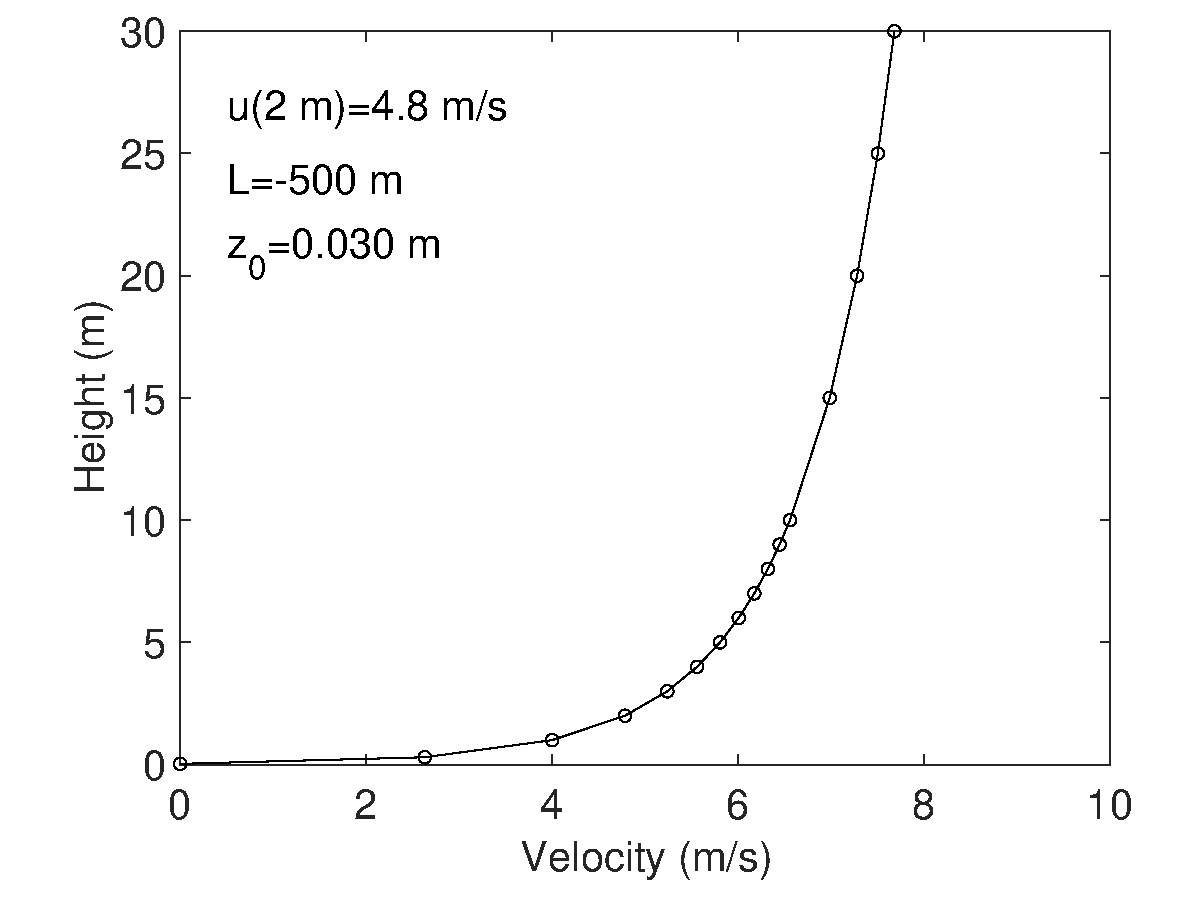
\includegraphics[width=.45\textwidth]{figures/vel_L=-500.pdf}
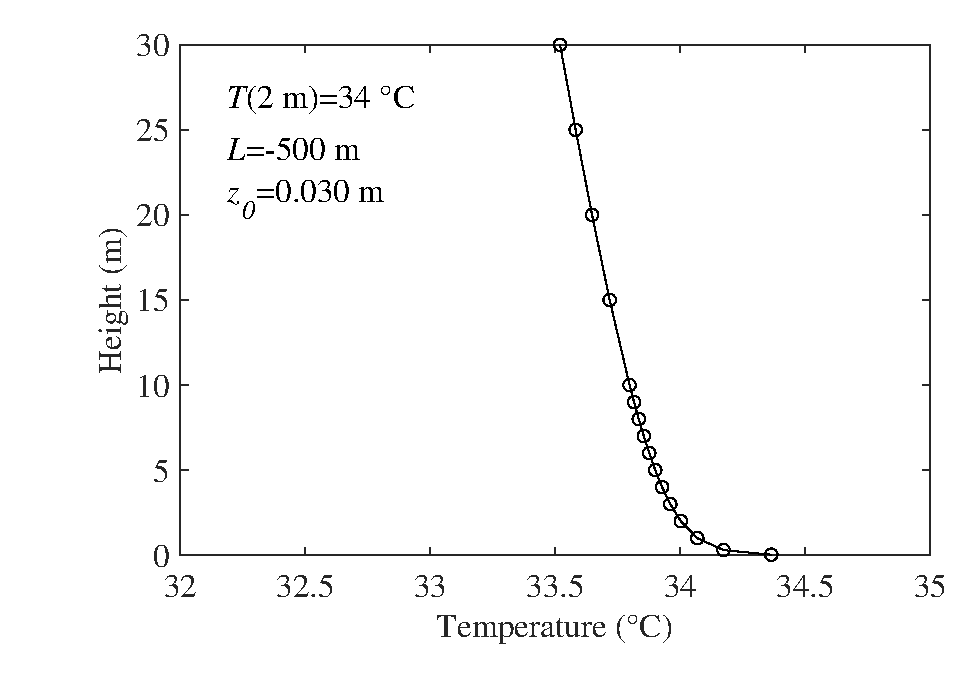
\includegraphics[width=.45\textwidth]{figures/tmp_L=-500.pdf}
\caption{Monin-Obukhov velocity and temperature profiles for inflow boundary conditions.  Here parameters are $L=-500\;\mathrm{m}$, $z_0=0.03\;\mathrm{m}$, and $u_r=4.8\;\mathrm{m/s}$ and $T_r=34\;^\circ\mathrm{C}$.} 
\label{fig:MOprofs}
\end{figure}

\subsection{Turbulent Inflow Conditions}

It is possible in FDS to superimpose synthetic turbulence on a specified inlet profile utilizing Jarrin's synthetic eddy method (SEM) \cite{Jarrin:2008}.  An example verification case is presented in Fig.~\ref{fig:semprofs}.  The left image of the figure shows contours of the normal component of velocity at the inlet.  The plot on the right shows the mean and rms profiles compared to the specified inlet parameters.  The domain is 20 m in the streamwise dimension by 12 m in the spanwise by 13 m in height.  In The turbulence intensity is set to 10 \% and the turbulence integral length scale is set to 3 m.  The specified MO parameters are $L=-667\;\mathrm{m}$, $z_0=0.022\;\mathrm{m}$, and $u_r=10\;\mathrm{m/s}$ and $T_r=20\;^\circ\mathrm{C}$ at reference height of 10 m.  The simulation runs for 60 seconds with statistics collected over the last 30 seconds.  The lateral, top, and downstream boundaries are set to ``open'' pressure boundaries as discussed in the next section.

\begin{figure}[ht]
\centering
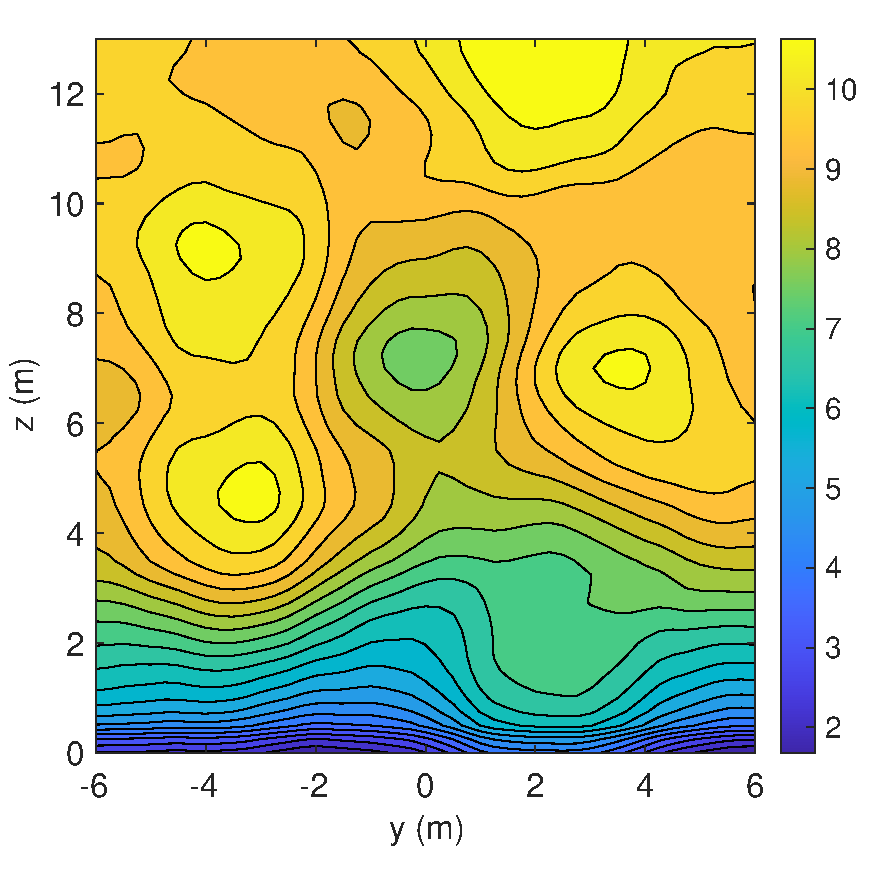
\includegraphics[width=0.45\textwidth,valign=c]{figures/sem_open_wind_contours.pdf}
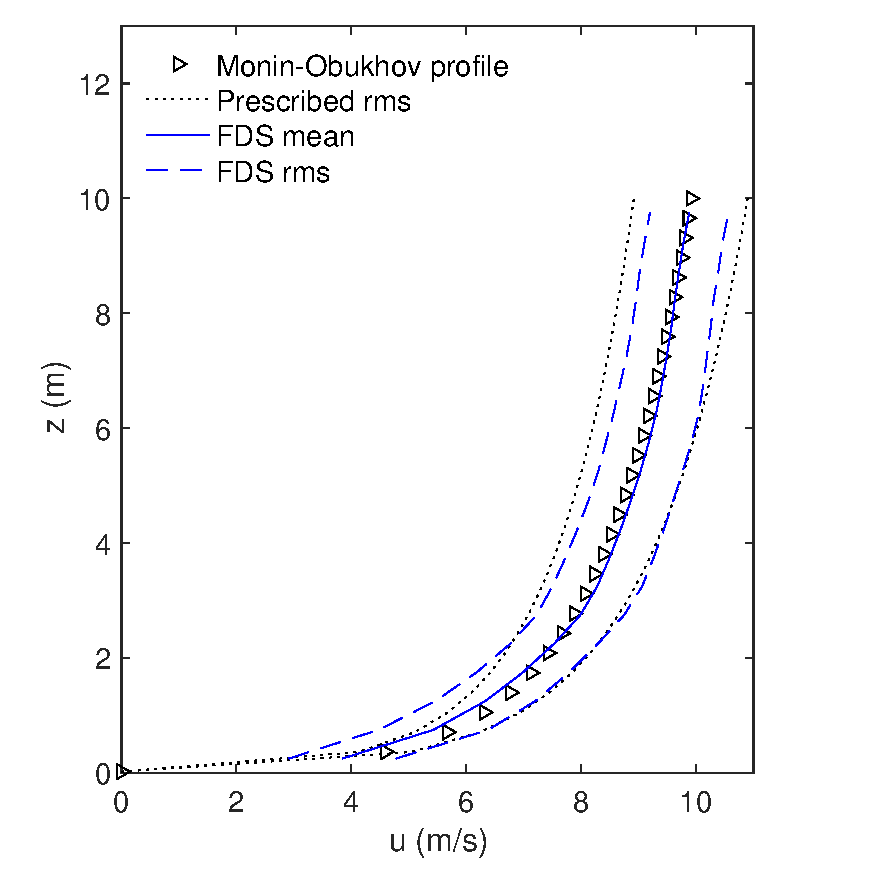
\includegraphics[width=0.5\textwidth,valign=c]{figures/sem_open_wind_u_prof.pdf}
\caption{Example of inflow synthetic turbulence superimposed on a Monin-Obukhov boundary layer profile. Contours of the normal component of velocity at the domain inlet taken at time midway through the simulation (left); mean and rms profiles along the inlet compared with specified profiles (right).  The MO parameters are $L=-667\;\mathrm{m}$, $z_0=0.022\;\mathrm{m}$, and $u_r=10\;\mathrm{m/s}$ and $T_r=20\;^\circ\mathrm{C}$ at reference height of 10 m.  SEM turbulence parameters were 10 \% turbulence intensity and an eddy integral length scale of 3 m.}
\label{fig:semprofs}
\end{figure}

Other approaches to imposing boundary layer turbulence are possible (e.g., \cite{Munoz-Esparza:2014}).  The cases presented later in this paper do not utilize SEM since detailed data on the turbulence statistics were not available.

\subsection{Pressure Boundary Values}

The Poisson equation for $H$, Eq.~(\ref{it:FSPoisson}), links the momentum equation with mass and energy in the low-Mach flow algorithm.  The boundary conditions for this equation determine the inflow and outflow velocity component values.  Let $\mathbf{n}$ denote a unit normal vector pointing \emph{into} the domain.  Boundary values at an interface are denoted with a subscript ``$I$''.  Then $\mathbf{u}_I\cdot\mathbf{n}>0$ is an inflow and $\mathbf{u}_I\cdot\mathbf{n}<0$ is an outflow condition.

At an inflow, generally the mean viscous and convective forces are small and we make use of a simplified momentum equation that approximates $\partial u_i/\partial t = -\partial H/\partial x_i$.  Let $u$ denote the $x$-component of velocity and consider an interface normal to $x$ pointing into the domain.  The prescribed external wind field velocity component at height $z$ and time $t$ (discussed above in Sec.~\ref{sec:veltmpprof}) is denoted $u_{wind}(z,t)$.  Using a one-sided difference for $H$ and an explicit Euler approximation of the velocity time derivative, the boundary value for $H$ may be written as 
\begin{equation}
\label{eq:Hin}
H_I = H_{I\pm\frac{1}{2}}^n \pm \frac{\Delta x}{2}\left[\frac{u_{wind,I}(z,t) - u_I^n}{\Delta t}\right] \quad \mbox{if} \quad \mathbf{u}_I\cdot\mathbf{n}>0
\end{equation}
At an outflow boundary, $H$ is set equal to the local kinetic energy per unit mass from the cell just upwind of the boundary:
\begin{equation}
\label{eq:Hout}
H_I = \frac{1}{2}(\bar{u}^n \bar{u}^n + \bar{v}^n \bar{v}^n + \bar{w}^n \bar{w}^n)_{I\pm\frac{1}{2}} \quad \mbox{if} \quad \mathbf{u}_I\cdot\mathbf{n}<=0
\end{equation}
The overbar on the velocity components denotes a linear interpolation of the primitive staggered component values to the cell center.

\section{Numerical Experiments} \label{sec:numexp}


\subsection{Flat Terrain Fire Spread}  \label{sec:simexp}

In July and August of 1986, the Commonwealth Scientific and Industrial Research Organisation (CSIRO) of Australia conducted controlled grassland fire experiments near Darwin, Northern Territory~\cite{Cheney:IJWF1993}. July and August are in the middle of the dry season when the grasses are fully cured (dried) and the weather is warm and dry. The experiments were conducted on flat plots measuring 100~m by 100~m, 200~m by 200~m, or 200~m by 300~m. Two cases have been simulated. Case~C064 was conducted on a 100~m by 100~m plot of kerosene grass ({\it Eriachne burkittii}); Case~F19 was conducted on a 200~m by 200~m plot of kangaroo grass ({\it Themeda australis}).

Two of these experiments were originally simulated with FDS by Mell~et~al.~\cite{Mell:IJWF2007} using a form of the Boundary Fuel Model. Now these two experiments are also simulated using the Lagrangian Particle Model and the Level Set Model. The level set simulations of Case~C064 use fuel index 1 (Short Grass) and for Case~F19, fuel index 3 (Tall Grass)~\cite{Rothermel:1972,Albini:1976}.

Measured bulk properties of the grasses burned in the two experiments are listed in Table~\ref{Properties_Grasses}. Properties that were not measured are listed in Table~\ref{Assumed_Properties_Grasses}. These assumed properties are typically for wood or cellulosic fuels. The moisture is modeled as water. The grass is assumed to be composed primarily of cellulose.

\begin{figure}[p]
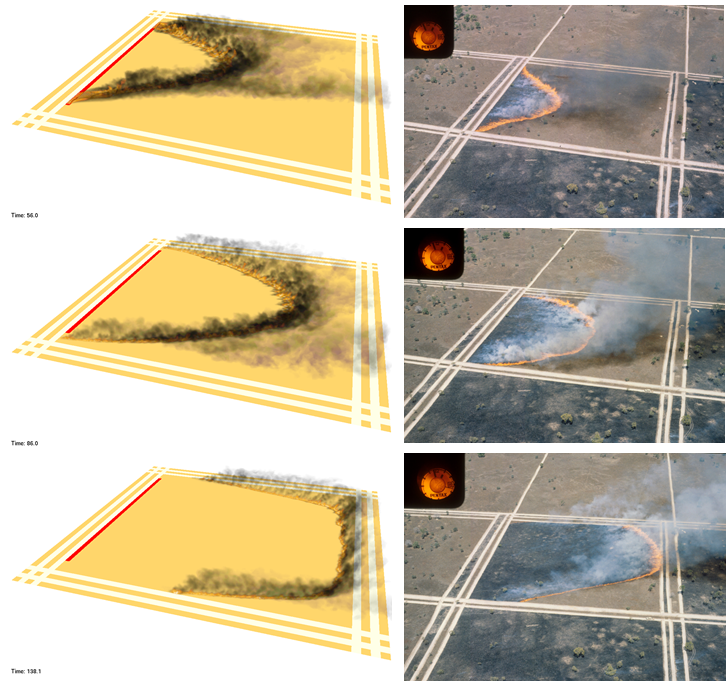
\includegraphics[width=\textwidth]{figures/F19_collage.png}
\caption{Photographs of the experiment and snapshots of the simulation of CSIRO Grassland Fire F19, 56~s, 86~s, and 138~s following ignition.}
\label{F19}
\end{figure}

\begin{figure}[ht]
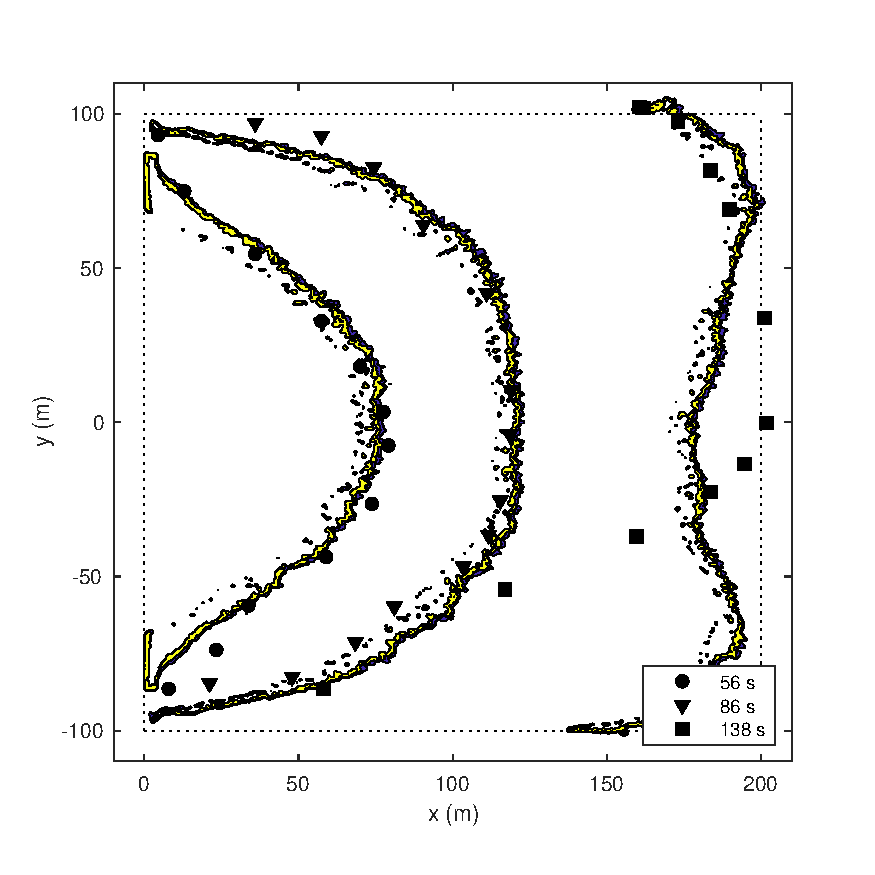
\includegraphics[width=0.49\textwidth]{figures/Case_F19_flame_position.pdf}
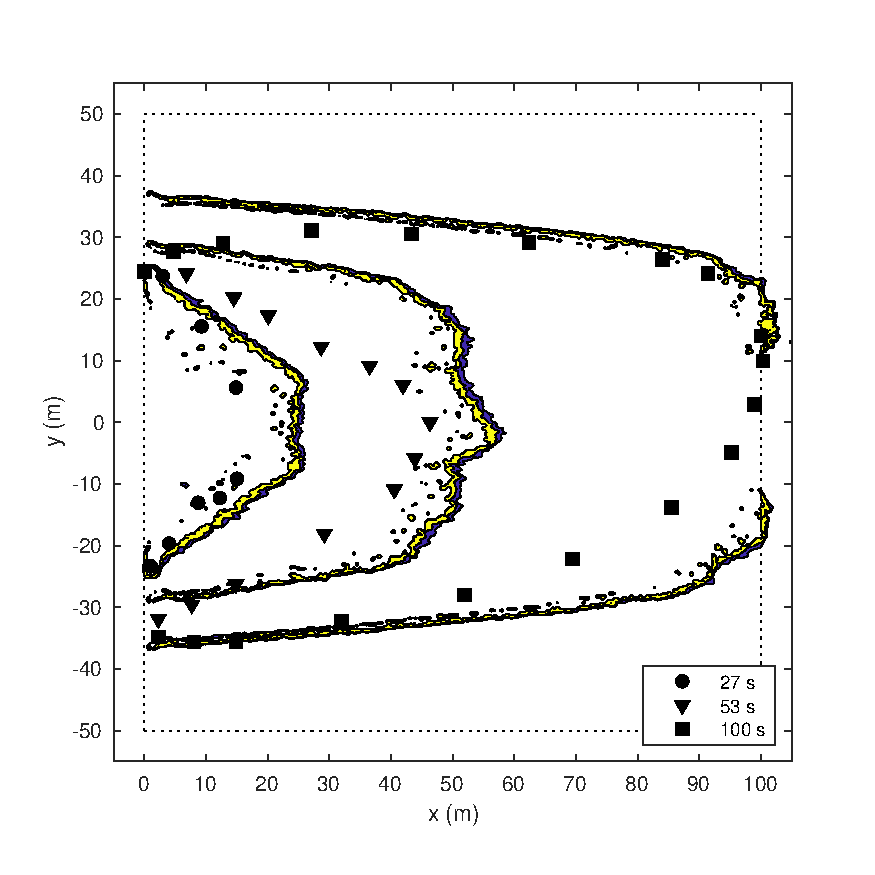
\includegraphics[width=0.49\textwidth]{figures/Case_C064_flame_position.pdf}
\caption{Contours of heat release rate in a plane near the surface compared to observations of CSIRO Grassland Fires F19 (left) and C064 (right).  FDS contour times for Case C064 have been shifted uniformly by 10 s to line up the initial head fire observation and compare the subsequent spread rate.}
\label{fig:CaseF19_contours}
\end{figure}

Snapshots of the Lagrangian particle simulation of Case~F19 compared to photographs of the experiment are shown in Fig.~\ref{F19}. The plot of grass is 200~m by 200~m and the computational domain is 240~m by 240~m by 20~m high. The grid cells are 0.5~m cubes. The domain is subdivided into 36 individual meshes and run in parallel. A blade of grass is represented by a single cylindrically-shaped particle within a grid cell. The radius of the cylinder is derived from the measured surface area to volume ratio of the grass. Each simulated blade of grass represents many more actual blades of grass. The weighting factor is determined from the measured bulk mass per unit area. The fires in the experiments were ignited by two field workers carrying drip torches walking in opposite directions along the upwind boundary of the plot (the red strip in Fig.~\ref{F19}). In FDS, this action was modeled using a specified spread rate along the strip.

\begin{table}[ht]
\begin{center}
\caption[Measured properties for the CSIRO Grassland Fire cases]{Measured properties for the CSIRO Grassland Fire cases~\cite{Cheney:IJWF1993}.}
\label{Properties_Grasses}
\begin{tabular}{|l|c|c|c|}
\hline
Property                        & Units         & Case F19      & Case C064     \\ \hline \hline
Wind Speed                      & m/s           & 4.8           & 4.6           \\ \hline
Ambient Temperature             & $^\circ$C     & 34            & 32            \\ \hline
Surface Area to Volume Ratio    & m$^{-1}$      & 12240         & 9770          \\ \hline
Grass Height                    & m             & 0.51          & 0.21          \\ \hline
Bulk Mass per Unit Area         & kg/m$^2$      & 0.313         & 0.283         \\ \hline
Moisture Fraction               & \%            & 5.8           & 6.3           \\ \hline
Measured ROS                    & m/s           & 1.5           & 1.1           \\ \hline
Calculated ROS, Particle Method (0.25 m, 0.5 m, 1.0 m resolution) & m/s           & 1.4, 1.3, 1.4           & 1.1, 1.2, 1.2          \\ \hline
Calculated ROS, Boundary Fuel Method (0.25 m, 0.5 m, 1.0 m resolution) & m/s      & 1.5, 1.4, 1.7           & 1.3, 1.3, 1.3           \\ \hline
Calculated ROS, Level Set Method (5 m, 10 m, 20 m resolution) & m/s          & 1.1, 1.1, 1.2          & 0.4, 0.5, 0.8          \\ \hline
\end{tabular}
\end{center}
\end{table}

\begin{figure}[p]
\begin{tabular*}{\textwidth}{l@{\extracolsep{\fill}}r}
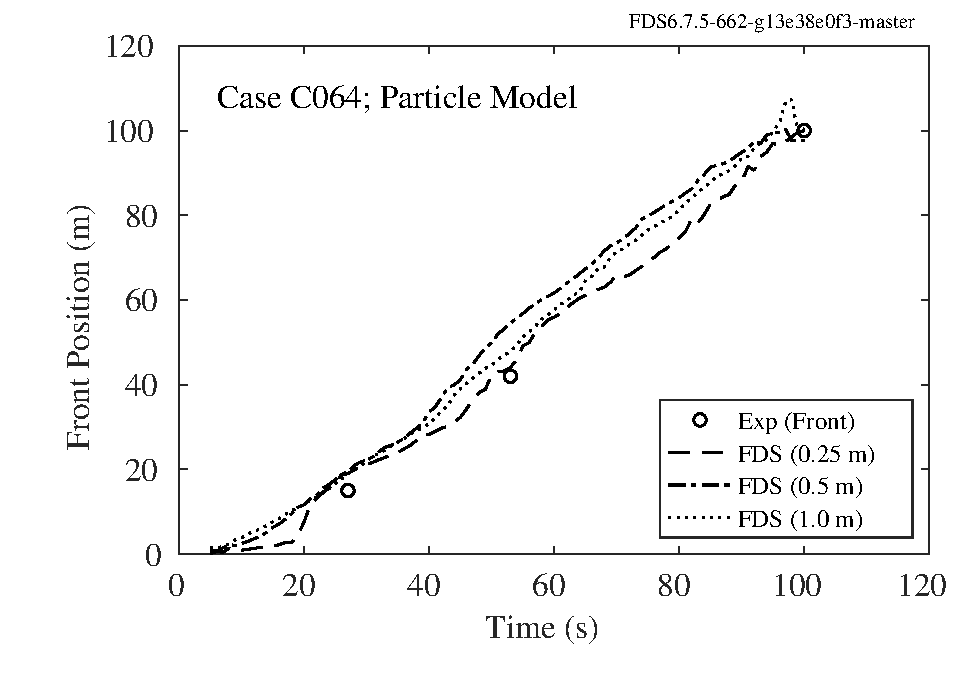
\includegraphics[height=2.2in]{figures/Case_C064} &
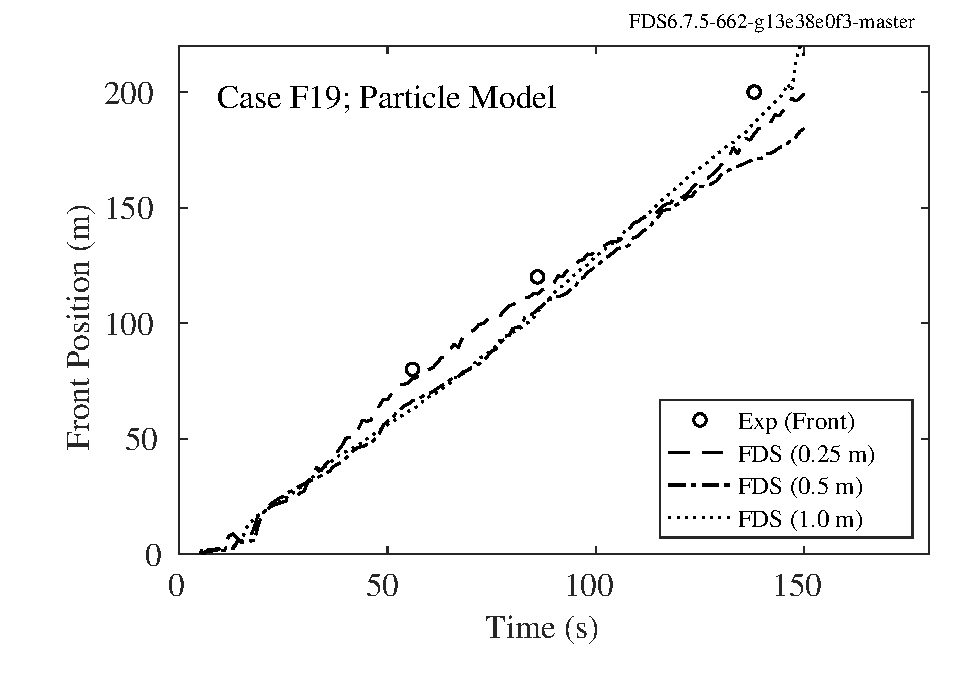
\includegraphics[height=2.2in]{figures/Case_F19} \\
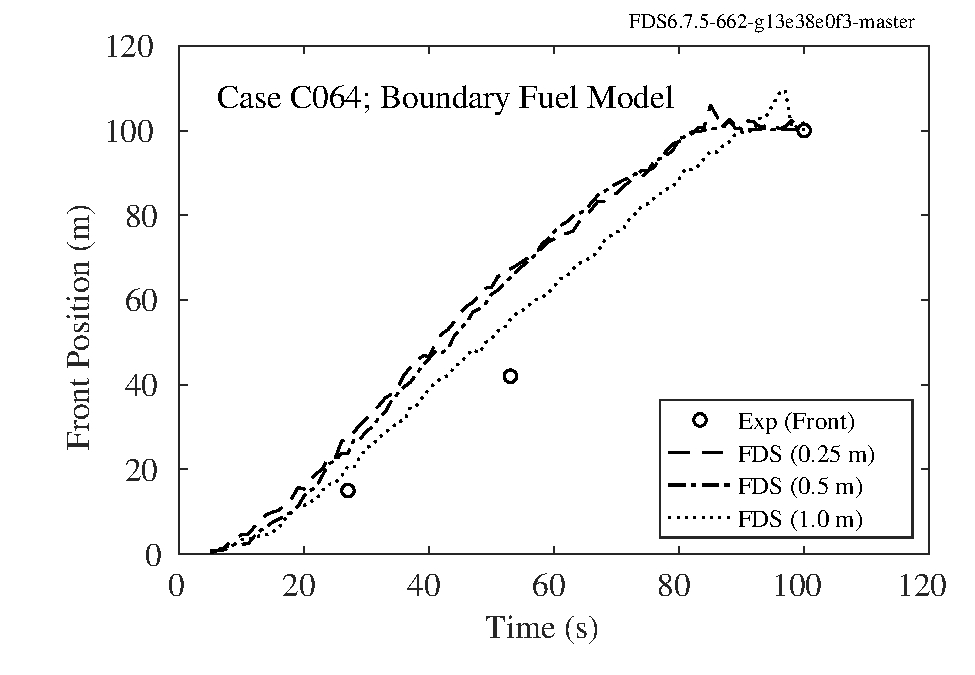
\includegraphics[height=2.2in]{figures/Case_C064_BFM} &
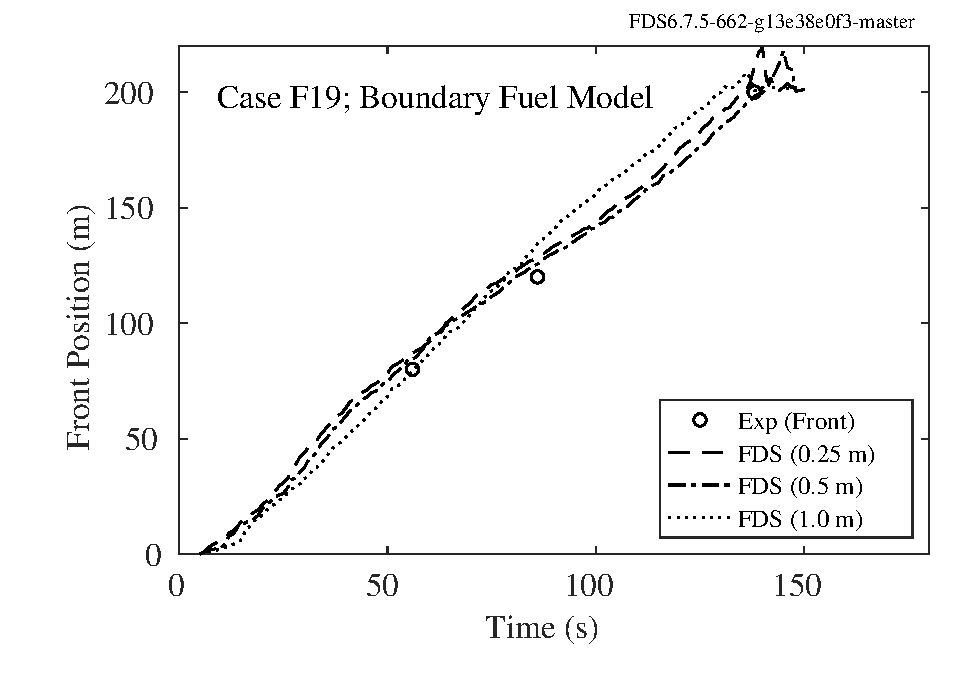
\includegraphics[height=2.2in]{figures/Case_F19_BFM} \\
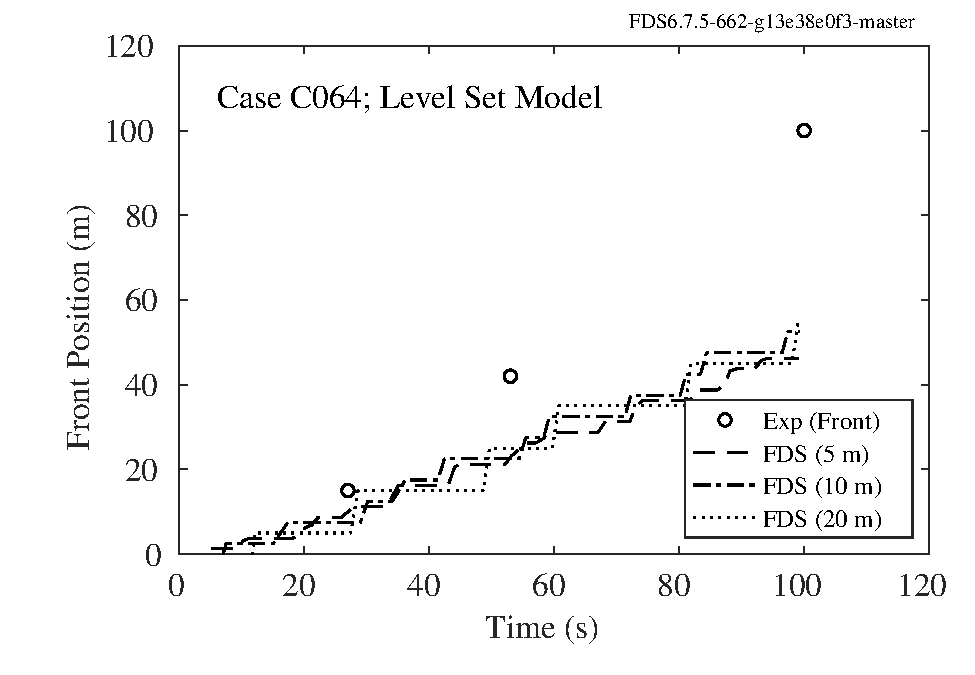
\includegraphics[height=2.2in]{figures/Case_C064_LS}  &
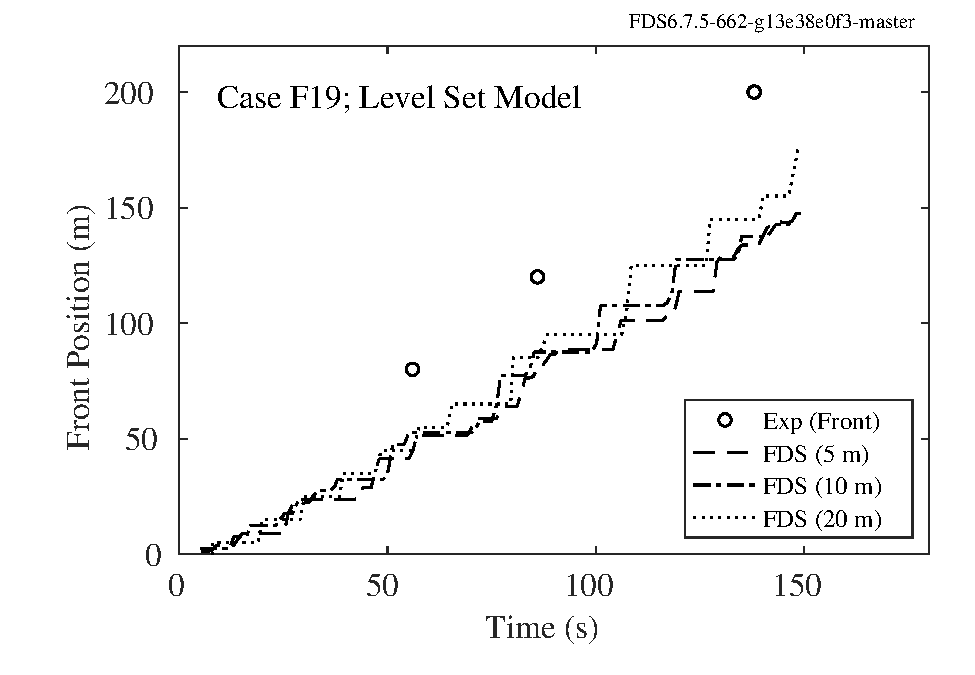
\includegraphics[height=2.2in]{figures/Case_F19_LS}
\end{tabular*}
\caption{Comparison of the measured and predicted fire front position for the CSIRO Grassland Fires using three different methods of fire spread.}
\label{CSIRO}
\end{figure}

The simulations have been conducted with the three different fire spread models, and each case has been run with three levels of spatial resolution. The simulations using the Particle and Boundary Fuel Models have been run with cubic grid cells that are 0.25~m, 0.5~m, and 1~m on a side. The simulations using the Level Set Model are run with cells of 5~m, 10~m, and 20~m. The predicted rates of spread for the two cases are listed in Table~\ref{Properties_Grasses} and shown graphically in Fig.~\ref{CSIRO}. For these simulations, the rate of spread predicted by the Particle and Boundary Fuel Models are comparable to the measured rate of spread while the level set method under-predicts the RoS. The under-prediction by the level set simulations is a consequence of the choice of fuel model, and one should not draw any conclusions as to the performance of level sets versus the other two rate of spread methods.

It is difficult to compare the Particle and Boundary Fuel simulations with those conducted by Mell et al. in 2007~\cite{Mell:IJWF2007}. The underlying numerical model, FDS, has undergone a major revision over the past decade, changing the basic finite-difference scheme, boundary conditions, drag modeling, and so on, and the vegetation-specific models have changed as well, most notably the charring reaction. In addition, the amount of information about the grasses and field conditions is limited, and the thermal and kinetic parameters are gleaned from various sources and are generally average values over a wide range of vegetation types. A sensitivity study~\cite{McGrattan:CI2017} for the particle model simulations reveals that near-surface wind speed is the has the most direct effect on the RoS, and the combined effect of the dozens of thermal, kinetic, and numerical parameters would certainly explain the difference in RoS. 


\begin{table}[ht]
\begin{center}
\caption[Assumed properties for dry grass and soil]{Assumed properties for various types of dried grass and soil. Note that the Pyrolysis Temperature is taken to be the temperature at which the mass loss rate peaks in the TGA experiments of Morvan and Dupuy~\cite{Morvan:CF2004}.}
\label{Assumed_Properties_Grasses}
\begin{tabular}{|l|c|c|c|}
\hline
Property                        & Units                 & Value                     & Reference                             \\ \hline \hline
Chemical Composition            & --                    & C$_6$H$_{10}$O$_5$        & Assumption                            \\ \hline
Heat of Combustion              & kJ/kg                 & 15600                     & \cite{Susott:FS1982}                  \\ \hline
Soot Yield                      & kg/kg                 & 0.015                     & \cite{SFPE:Tewarson}                  \\ \hline
Char Yield                      & kg/kg                 & 0.2                       & \cite{Susott:FS1982}                  \\ \hline
Specific Heat                   & kJ/(kg$\cdot$K)       & 1.5                       & Various sources                       \\ \hline
Conductivity                    & W/(m$\cdot$K)         & 0.1                       & Assumption                            \\ \hline
Density                         & kg/m$^3$              & 512                       & \cite{Rothermel:1972}                 \\ \hline
Heat of Pyrolysis               & kJ/kg                 & 418                       & \cite{Morvan:CF2004}                  \\ \hline
Pyrolyis Temperature            & $^\circ$C             & 200                       & \cite{Morvan:CF2004}                  \\ \hline \hline
Obukhov Length                  & m                     & -500                      & Assumption                            \\ \hline
Aerodynamic Roughness Length    & m                     & 0.03                      & Assumption                            \\ \hline
Drag Coefficient                & --                    & 2.8                       & \cite{Falkenstein-Smith:2018}         \\ \hline \hline
Soil Specific Heat              & kJ/(kg$\cdot$K)       & 2.0                       & \cite{Farouki:1981}                   \\ \hline
Soil Conductivity               & W/(m$\cdot$K)         & 0.25                      & \cite{Farouki:1981}                   \\ \hline
Soil Density                    & kg/m$^3$              & 1300                      & \cite{Farouki:1981}                   \\ \hline

\end{tabular}
\end{center}
\end{table}






\subsection{Complex Terrain Fire Spread}  
\label{sec:cogo}

This section presents an example of the methodologies discussed in the paper. It is notable because it considers an actual fire that occurred in the urban-wildland interface, which presents a challenge for a fire spread model because the surface vegetation is mixed with the built environment.

At approximately 23:00 (local time) on March 25, 2019, a wildfire started in the seaside town of Cogoleto, near Genova, Italy. Strong winds, gusting up to 100~km/h from the North, spread the fire from its ignition point due to a faulty electric line on a ridge above the town towards the sea. Several houses were destroyed, hundreds of residents had to be evacuated, the firefighter crews worked for three days to tame the flames, no casualties were reported.

\begin{figure}[ht]
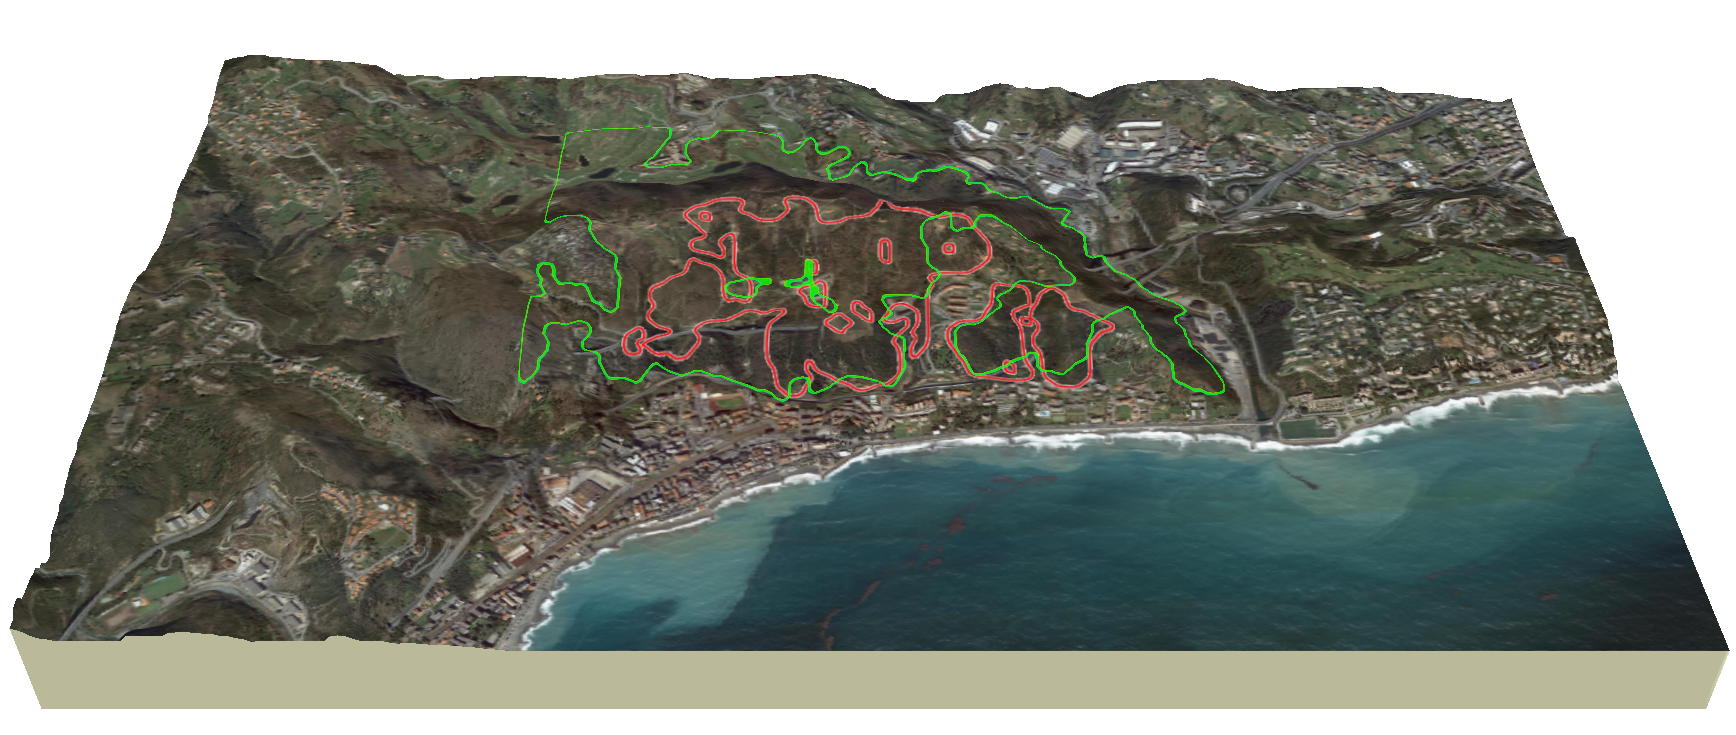
\includegraphics[width=\textwidth]{figures/cogoleto_fire_2019_ls4_1000.png}
\caption{Satellite photograph of the region where the Cogoleto Fire occurred. The area outlined in red is the extent of the actual fire; green is the simulation.}
\label{Cogoleto_satellite}
\end{figure}

Shown in Fig.~\ref{Cogoleto_satellite} are the results of a level set simulation of the fire superimposed on a satellite photograph of the area and the outline of the extent of the actual fire.

The computational domain is assembled using the open-source GIS (Geographic Information System) program called QGIS~\cite{QGIS}, extended by the qgis2fds~\cite{qgis2fds} plugin. The open-source qgis2fds plugin was specifically developed in the framework of the WUIFI-21 project\footnote{WUIFI-21: {\it High fidelity computational fluid dynamics modeling of forest fires for Wildland-Urban Interface communities resilience and protection}, an Italy-US research project financed by the Italian Ministry of Foreign Affairs and International Cooperation} for facilitating the use of geographical data for forest fire simulation and smoke pollutants dispersion in FDS.

The wind speed and direction are based on a single weather station near the point of ignition. The vegetation type is provided by a database maintained at the CIMA\footnote{International Centre on Environmental Monitoring.} Research Foundation, derived from regional forest management maps. In the simulation, the single point wind data is taken as the prevailing wind, and the local wind field is obtained via a CFD computation. The fire is simulated based on the position of the level set front; that is, when the front arrives at a given location, a fire is ignited and burns for a duration of time consistent with the specified fuel loading of that particular point on the map. 

The extent of the simulated fire, shown in green in Fig.~\ref{Cogoleto_satellite}, is greater than the actual fire, shown in red. This is not surprising given that the simulation does not include fire suppression and the rate of spread of the level set front is determined empirically for vegetation that may not exactly resemble that of this particular region. 

The simulation results have been compared with those obtained from CIMA Propagator~\cite{Trucchia:2020}, an experimental propagation model that has provided several European civil protection organizations with real-time fire predictions since 2009. The model has been implemented by the CIMA Foundation, its propagation model is based on stochastic cellular automata.

The two models produce a qualitatively similar patterns of fire spread, mainly because the vicinity of the fire has numerous areas that are considered ``non-combustible,'' that is, devoid of vegetation or structures. This points out the problem of ``validating'' wildfire models. The simulations of the flat terrain grassland fire experiments described in the previous section match fairly well the observed fire behavior, but in these cases, the vegetation is uniform and fairly well described in terms of its mass loading and geometrical characteristics, the terrain is flat and of relatively small area, the wind is steady, and the experiment lasts a few minutes. In a real fire, none of this will be true. The detailed physics of the fire are not resolvable on a relatively coarse grid, the vegetation is inhomogeneous, sparse, and sometimes unknown, the weather conditions are varying, there are suppression efforts with water and the setting of backfires, and the fires can burn for days. All of which raise the question as to what level of physical fidelity ought to be required in these models. The strategy that has been adopted in FDS is to accommodate simulation options ranging from a level set calculation of fire spread over tens of kilometers that can be run in minutes, similar to models like BEHAVE developed by the U.S. Forest Service, all the way to detailed simulations of fire spread at sub-meter resolution for relatively short time periods (minutes to hours) and small areas (tens of hectares). As was the case for models developed for building fires thirty years ago, it is not clear at the moment exactly how these wildland fire models will be used in the future. The best strategy is to advance the various modeling options until a clear path forward becomes apparent.


\section{Summary} \label{sec:summary}

The numerical methods described in this paper span the range of length scales from tens of centimeters to tens of kilometers. Obviously, these techniques support differing descriptions of the underlying fire physics, but all can be embedded within the same code base. This allows researchers to combine the different techniques in ways that were not possible when separate codes were maintained by separate organizations. With FDS, one can simulate 24 hours of fire spread in minutes of computation time using the level set function and a wind field that varies only temporally, not spatially, with no fire-atmospheric coupling. At the same time, using the same set of input parameters, one can simulate the fire at far greater resolution with much greater physical fidelity, albeit for shorter time periods and spatial extent.





\reftitle{References}


\externalbibliography{yes}
\bibliography{Vanella_Article_Atmosphere_2020,LOFM_Workshop_References,FDS_refs}


% The following MDPI journals use author-date citation: Arts, Econometrics, Economies, Genealogy, Humanities, IJFS, JRFM, Laws, Religions, Risks, Social Sciences. For those journals, please follow the formatting guidelines on http://www.mdpi.com/authors/references
% To cite two works by the same author: \citeauthor{ref-journal-1a} (\citeyear{ref-journal-1a}, \citeyear{ref-journal-1b}). This produces: Whittaker (1967, 1975)
% To cite two works by the same author with specific pages: \citeauthor{ref-journal-3a} (\citeyear{ref-journal-3a}, p. 328; \citeyear{ref-journal-3b}, p.475). This produces: Wong (1999, p. 328; 2000, p. 475)




%% for journal Sci
%\reviewreports{\\
%Reviewer 1 comments and authors’ response\\
%Reviewer 2 comments and authors’ response\\
%Reviewer 3 comments and authors’ response
%}

%%%%%%%%%%%%%%%%%%%%%%%%%%%%%%%%%%%%%%%%%%
\end{document}

